\documentclass[10pt]{beamer}
\usepackage[utf8]{inputenc}
\usepackage[french]{babel}
\usepackage[T1]{fontenc}
\usepackage{beamerthemesplit}
\usepackage{graphics,epsfig, subfigure}
\usepackage{url}
\usepackage{siunitx}
\usepackage{fourier}
\usepackage{tikz}
\usepackage{numprint}

\DeclareSIUnit\year{yr}

\definecolor{jd_blue0}{rgb}{0.51,0.34,1.00}
\definecolor{jdbishop}{rgb}{0.27,0.14,0.29}
\definecolor{jddarkbl}{rgb}{0.18,0.14,0.29}
\definecolor{jd_brown}{rgb}{0.29,0.14,0.14}
\definecolor{jd_green}{HTML}{096F35}
\definecolor{jdorange}{rgb}{1.00,0.55,0.00}
\definecolor{jdredred}{rgb}{0.50,0.00,0.00}
\definecolor{SchoolColor}{rgb}{0.145,0.666,1}
\definecolor{pheniics}{HTML}{1a899c}
\definecolor{pheniics_purple}{HTML}{64003d}
\definecolor{chaptercolor}{gray}{0.8}
\mode<presentation>
{  \usetheme{PaloAlto}

  \setbeamercolor{palette primary}{bg=pheniics,fg=white}
  \setbeamercolor{palette secondary}{bg=pheniics_purple,fg=white}
  \setbeamercolor{palette tertiary}{bg=pheniics_purple,fg=white}
  \setbeamercolor{palette quaternary}{bg=pheniics_purple,fg=white}
  \setbeamercolor{palette sidebar primary}{fg=white}
  \setbeamercolor{palette sidebar secondary}{fg=white}
  \setbeamercolor{palette sidebar tertiary}{fg=pheniics_purple}
  \setbeamercolor{palette sidebar quaternary}{fg=pheniics_purple}
  \setbeamercolor{structure}{fg=pheniics} % itemize, enumerate, etc
  \setbeamercolor{section in toc}{fg=black}

  \useinnertheme{circles}
  \usefonttheme[onlymath]{serif}
  \setbeamercovered{transparent}
  \setbeamertemplate{blocks}[rounded][shadow=true]
  \setbeamertemplate{navigation symbols}{}
  \addtobeamertemplate{footline}{
    \usebeamercolor[fg]{author in sidebar}
    \vskip-1cm\hskip15pt
    \insertframenumber\,/\,\inserttotalframenumber\kern1em\vskip2pt%
  }
}
\setbeamercovered{invisible}
%\setbeamertemplate{background}{\includegraphics[width=1\textwidth]{natfak_baggrund.pdf}}

\graphicspath{{../Chapitre_1/pictures/}{../Chapitre_2/pictures/}{../Chapitre_3/pictures/}{../Chapitre_4/pictures/}{../Chapitre_5/pictures/}{../Front-back_covers/images/}{pictures/}}
 
\logo{
\includegraphics[width=1.5cm]{logo_CEA.png}}
\title[Le projet WA105]{Le projet WA105 : un prototype de Chambre à Projection Temporelle à Argon Liquide Diphasique utilisant des détecteurs LEMs}
\author{Présenté par \\ \textbf{Philippe Cotte} \\ \vspace{0.3cm} Sous la direction de \\ \textbf{E. Mazzucato}\vspace{-0.2cm}}
\institute{CEA Paris-Saclay \\ Université Paris-Saclay\vspace{-0.2cm}}
\date{\vspace{-0.2cm}17 Septembre 2019}

\def\TOO{\SI{4}{\tonne}}
\def\SSS{\SI{300}{\tonne}}
\def\threeL{\SI{3}{\liter}}
\def\dune{DU$\nu$E}
\def\checkmark{\tikz\fill[scale=0.4](0,.35) -- (.25,0) -- (1,.7) -- (.25,.15) -- cycle;}

\newenvironment{specialframe}
{
    \begingroup
    \advance\textwidth2cm % see beamerthemeGoettingen.sty for the number
    \hsize\textwidth
    \columnwidth\textwidth
    \begin{frame}[plain]
}
{
    \end{frame}
    \endgroup
}


\begin{document}

    {
        \usebackgroundtemplate{
\includegraphics[width=\paperwidth]{./pictures/1.pdf}}
        \begin{specialframe}
            \vspace{2cm}\hspace*{-1.8cm}\parbox[t]{\textwidth}{\titlepage}
        \end{specialframe}
    }
    \begin{specialframe}\tableofcontents\end{specialframe}

  \setcounter{framenumber}{0}
    {
    	\usebackgroundtemplate{
\includegraphics[width=\paperwidth]{./pictures/1.pdf}}
        \begin{specialframe}
            \vspace{2cm}\hspace*{-1.8cm}\parbox[t]{\textwidth}{
                \begin{center}
                    \begin{Huge}
                            \textcolor{pheniics_purple}{\textbf{Contexte}}
                    \end{Huge}
                \end{center}
            }
        \end{specialframe}
    }

  \section{Contexte}
    \subsection{WA105}

    \begin{frame}{Présentation du projet WA105}{Prototype la technologie DLArTPC}
        \begin{scriptsize}
            \begin{columns}
                \begin{column}{0.75\textwidth}
                    \centering
                    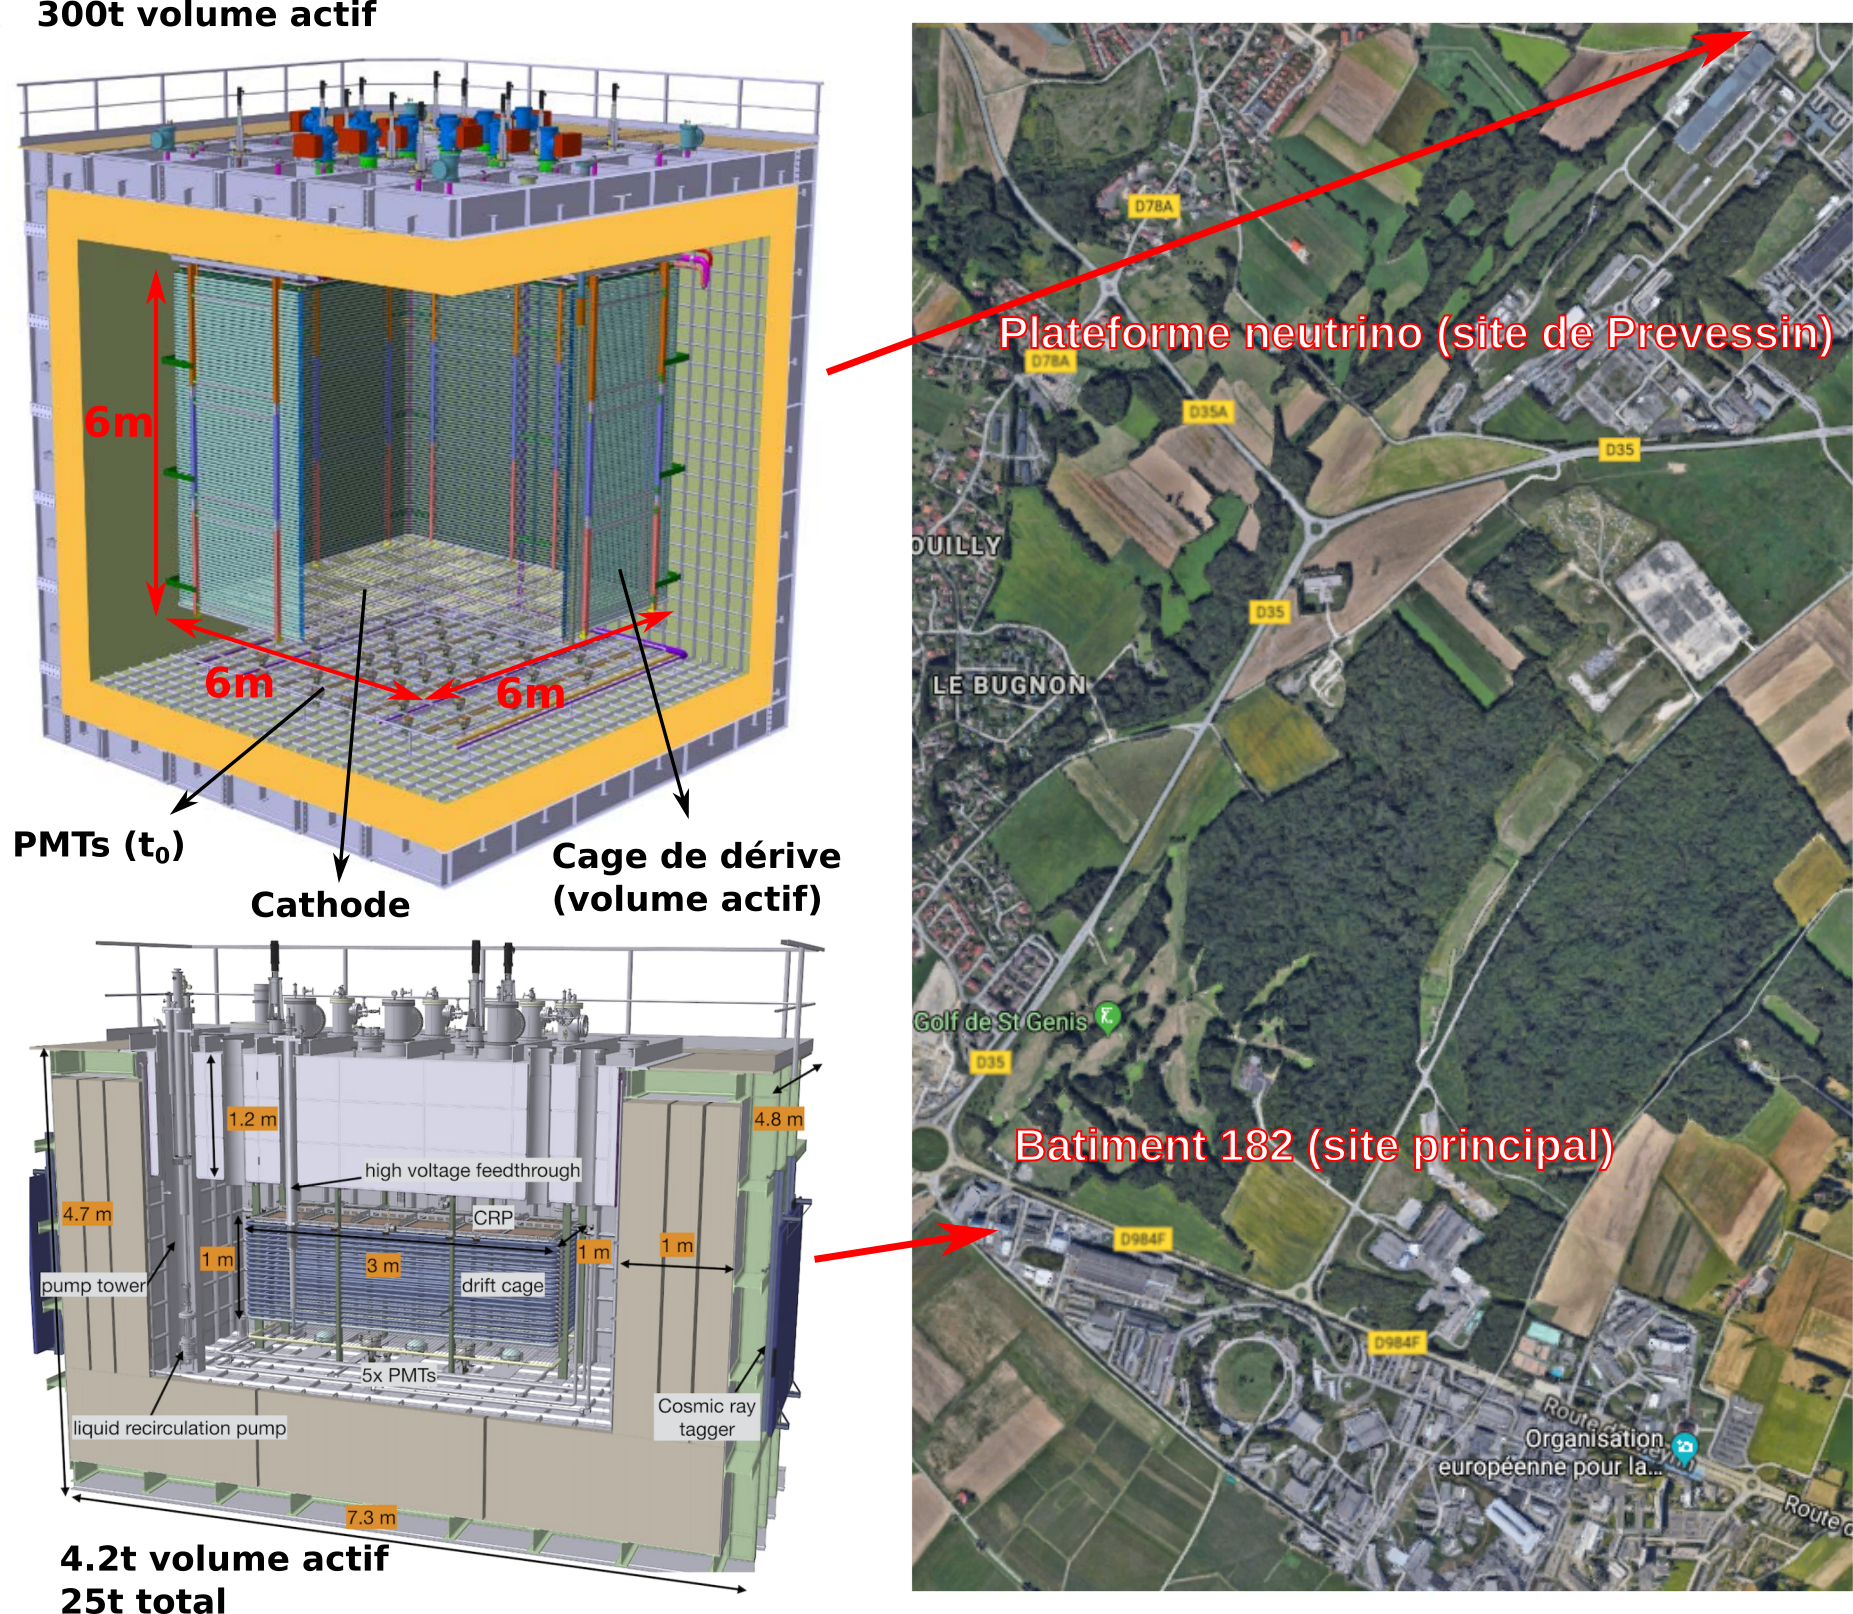
\includegraphics[height=0.9\textheight]{./pictures/wa105.png}
                \end{column}
                \begin{column}{0.25\textwidth}
                    \begin{itemize}
                        \item Prototype une nouvelle technologie : DLArTPC
                        \item Techno qui sera utilisée dans la future expérience \dune{} 
                        \item TPC utilisant de l'argon liquide
                        \item \textbf{+ : Double phase} \\$\to$ amplification du signal dans de l'argon gazeux
                    \end{itemize}
                \end{column}
            \end{columns}
        \end{scriptsize}
    \end{frame}

    \subsection{DU$\nu$E}

    \begin{frame}{DU$\nu$E : Deep Underground Neutrino Experiment}
        \begin{scriptsize}
            \centering
            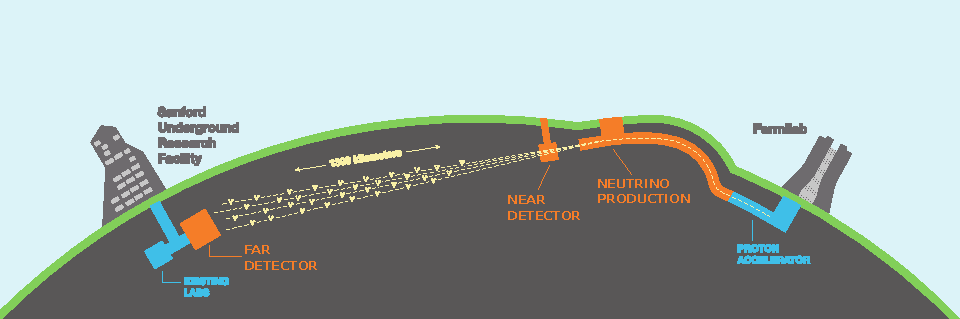
\includegraphics[width=\textwidth]{dune.pdf}\\
            \vspace{1cm}
            \begin{columns}
                \begin{column}{0.5\textwidth}
                    \begin{itemize}
                        \item[$\bullet$] Expérience d'\textbf{oscillation des neutrinos} d'accélérateur à longue ligne de base au USA, prévue pour fin 2026
                        \item[$\bullet$] Détectera dans le \textbf{Dakota du Sud} des $\nu$/$\overline{\nu}$ envoyés du \textbf{Fermilab} à \textbf{\SI{1300}{\kilo\meter}}.
                    \end{itemize}
                \end{column}
                \begin{column}{0.5\textwidth}
                    \textbf{Mesurera la probabilité de changement de saveur $P(\nu_{\mu}\to\nu_e)$ vs $E$ pour répondre à : }
                    \begin{itemize}
                        \item[$\bullet$] La symétrie CP est-elle violée dans le secteur leptonique?
                        \item[$\bullet$] Quel est l'ordre des masses des neutrinos?
                    \end{itemize}
                \end{column}
            \end{columns}
        \end{scriptsize}
    \end{frame}

    \begin{frame}{DU$\nu$E : Deep Underground Neutrino Experiment}
        \begin{scriptsize}
            \begin{columns}
                \begin{column}{0.6\textwidth}
                    \centering
                    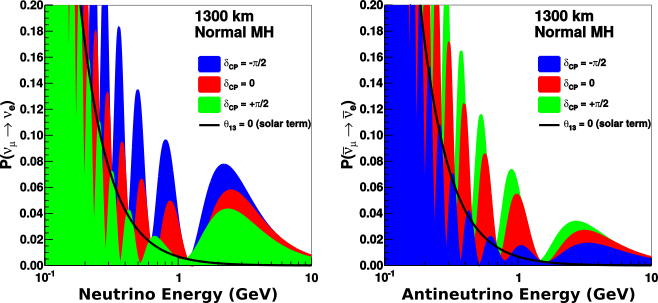
\includegraphics[width=\textwidth]{oscillation_CP.png}\\\vspace{0.2cm}
                    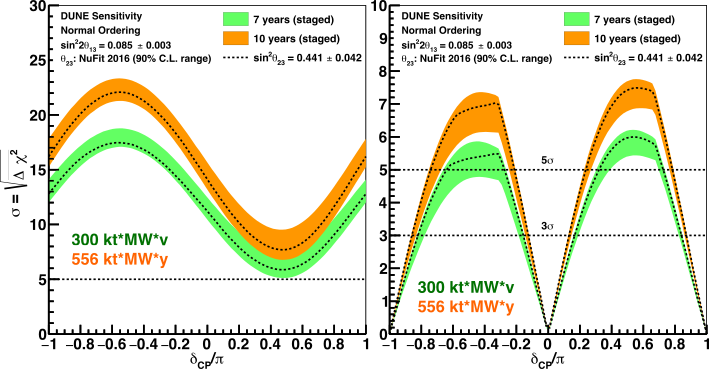
\includegraphics[width=0.95\textwidth]{sensitivities_2.png}\\
                    \begin{scriptsize}
                        Meilleures sensibilités seront présentées dans le TDR 2019
                    \end{scriptsize}
                \end{column}
                \begin{column}{0.4\textwidth}
                    \begin{itemize}
                        \item[$\bullet$]$\delta_{CP}\ne0$ et $\pi$ pourrait expliquer asymétrie \textcolor{red}{matière-antimatière} dans l'univers.\\
                        \item[$\bullet$] Plusieurs théories dépendent de \textcolor{red}{l'ordre des masses} des neutrinos.
                        \item[$\Rightarrow$] Les deux influencent la probabilité de changement de saveur.
                    \end{itemize}
                    \begin{scriptsize}
                        Pour mesurer \textcolor{red}{$P(\nu_{\mu}\to\nu_e)$ vs $E$}: \\
                        Besoin d'une reconstruction précise des interactions neutrinos pour atteindre $5\sigma$ pour la violation de CP.
                    \end{scriptsize}
                    \begin{itemize}
                        \item[$\bullet$] Reconstruction des traces en 3D
                        \item[$\bullet$] Calorimétrie
                        \item[$\bullet$] PID précis
                        \item[$\bullet$]Résolution en énergie $\leq$3\%
                    \end{itemize}
                \end{column}
            \end{columns}
        \end{scriptsize}
    \end{frame}

    \begin{frame}{DU$\nu$E : Deep Underground Neutrino Experiment}
        \begin{scriptsize}
            \begin{columns}
                \begin{column}{0.55\textwidth}
                    \centering Le détecteur lointain\\
                    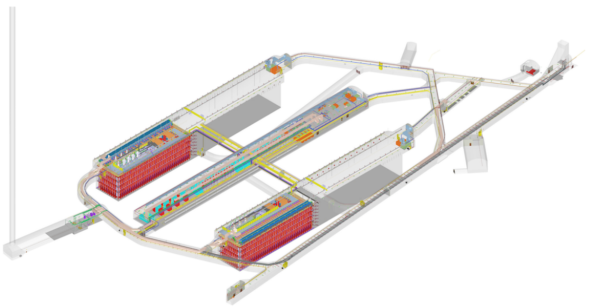
\includegraphics[width=0.8\textwidth]{./pictures/FD.png}\\
                    \centering Module simple phase\\
                    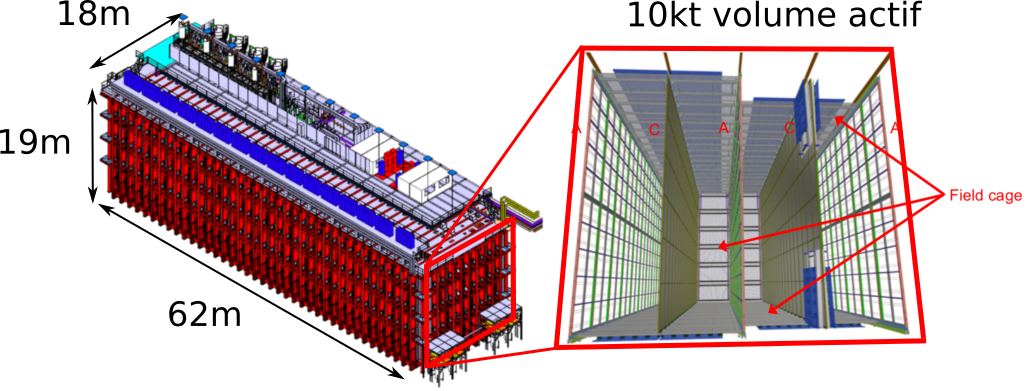
\includegraphics[width=\textwidth]{./pictures/module_SP.png}\\
                    \centering Module double phase (gauche) et intérieur de ProtoDU$\nu$E-DP (droite)\\
                    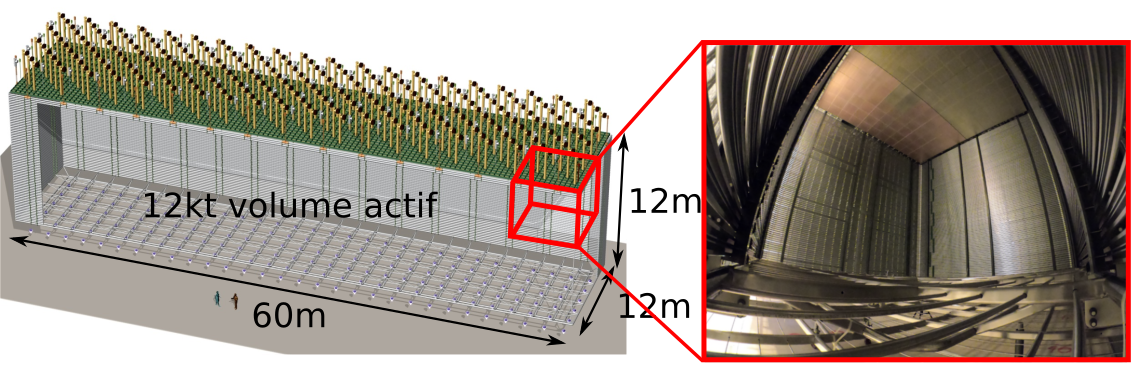
\includegraphics[width=0.9\textwidth]{./pictures/module_DP.png}
                \end{column}
                \begin{column}{0.45\textwidth}
                    \begin{itemize}
                        \item[$\bullet$] Détecteur lointain = 4 modules de LArTPC
                        \item[$\bullet$] 2 Simple Phase, 1 Double phase, 1 à déterminer
                    \end{itemize}
                    \textbf{Premier module simple phase} : construit de août 2024 à août 2025, rempli fin 2026.\\
                    \textbf{Début des prises de données} : fin 2026.\\
                    \textbf{Second module simple phase} : construit de sept. 2025 à oct. 2026, rempli début 2028.\\
                    \begin{itemize}
                        \item[$\Rightarrow$] \textbf{ProtoDU$\nu$E} teste les \textbf{2 versions} de la technologie LArTPC  à \SI{300}{\tonne} à la plateforme neutrinos du CERN.\\
                        \item[$\Rightarrow$]\textcolor{red}{\textbf{WA105/ProtoDU$\nu$E-DP}} test la version\\ \textcolor{red}{\textbf{Double Phase}} de la LArTPC.\\
                    \end{itemize}
                \end{column}
            \end{columns}
%            Timeline\\
        \end{scriptsize}
    \end{frame}


    \subsection[DLArTPC]{La technologie DLArTPC}

  {
    	\setlength\pdfpagewidth{12.8cm}%
    	\setlength\pdfpageheight{9.15cm}%
    	\usebackgroundtemplate{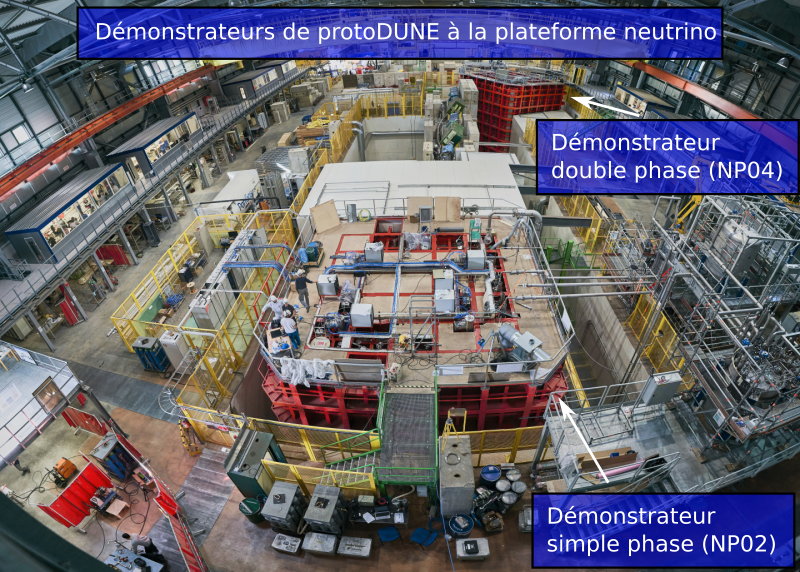
\includegraphics[width=\paperwidth]{nu_platform.png}}
    	\begin{frame}[plain]
    	\end{frame}
    }

  \begin{frame}{La technologie DLArTPC et le projet WA105}{L'argon liquide comme milieu de détection}
	  \begin{scriptsize}
    	\begin{columns}
    		\begin{column}{0.6\textwidth}
    			\centering
    			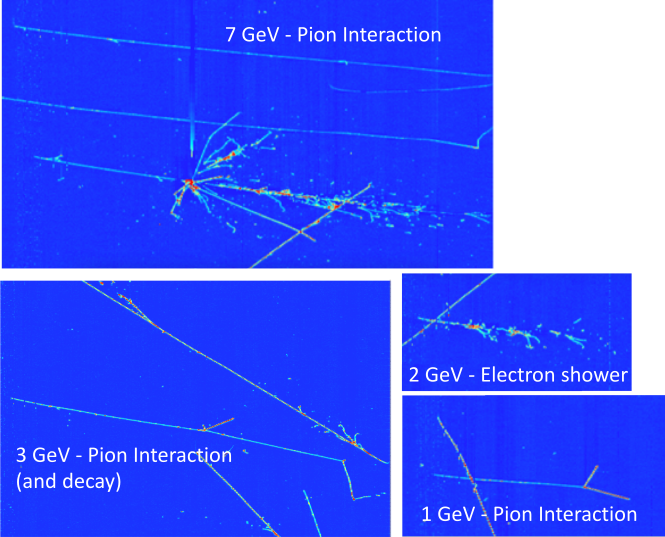
\includegraphics[width=\textwidth]{./pictures/SP_evt.png}\\
    			\flushleft
    			\begin{footnotesize}\textit{Événements dans protoDU$\nu$E-Simple Phase}\end{footnotesize}
    		\end{column}
    		\begin{column}{0.4\textwidth}
    			\begin{footnotesize}
    				\textbf{Pourquoi l'argon liquide?}
    			\end{footnotesize}
    			\begin{itemize}
    				\item[$\bullet$] MIP $\rightarrow\sim\SI{60000}{e^-\per\centi\meter}$. \\
    				(Bruit électronique $\sim \SI{1000}{e^-}$)
    				\item[$\bullet$] Gaz noble $\rightarrow$ ne piège pas les électrons.
    				\item[$\bullet$] Très bon trajectographe et calorimètre entièrement homogène.
    				\item[$\bullet$] Scintille au moment de l'ionisation $\rightarrow$ déclencheur et/ou $t_0$ \\ + transparent pour les photons  d'ionisation.
    				\item[$\bullet$] Dense (\SI{1.4}{\gram\per\centi\meter^3}).
    				\item[$\bullet$] Peu cher et abondant.
    			\end{itemize}
    			\begin{footnotesize}
	    			\textbf{$\Rightarrow$ Chambre à bulle électronique.}
	    		\end{footnotesize}
    		\end{column}
    	\end{columns}
	  \end{scriptsize}
    \end{frame}

    \begin{frame}{La technologie DLArTPC et le projet WA105}{Chambres à Projection Temporelle à Argon Liquide}
    	\begin{scriptsize}
    			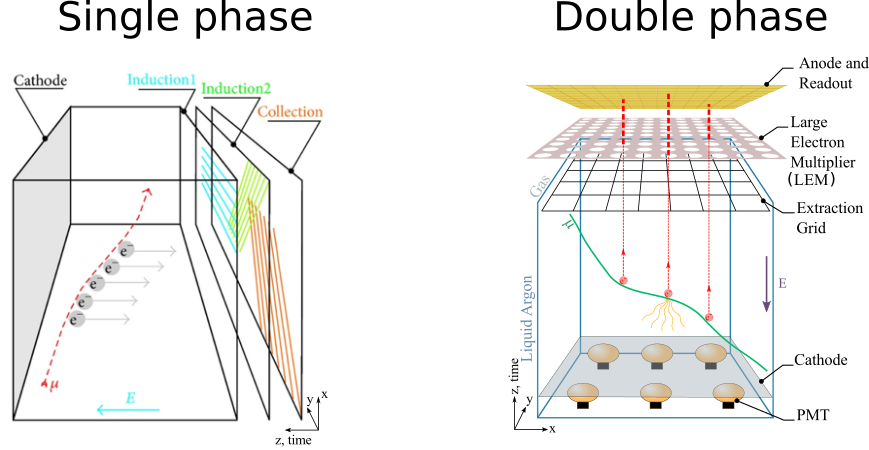
\includegraphics[width=0.9\textwidth]{tpcs.png}\\\vfill
    			\begin{columns}
    				\begin{column}{0.5\textwidth}
    					\begin{itemize}
    						\item[$\bullet$] Tout se passe dans l'argon liquide.
    						\item[$\bullet$] Mesure directe de l'énergie.
    						\item[$\bullet$] Les premiers événements de protoDU$\nu$E-SP ont été vus l'an dernier.
    					\end{itemize}
    				\end{column}\hfill
    				\begin{column}{0.5\textwidth}
    					\begin{itemize}
    						\item[$\bullet$] Amplification des charges dans le gaz\\$\Rightarrow$ Meilleur ratio signal/bruit.
    						\item[$\bullet$] Plus grande distances de dérive, moins de canaux de lecture, meilleure résolution spatiale.
    						\item[$\bullet$] Premières données en août 2019.
    					\end{itemize}
    				\end{column}
    			\end{columns}
    	\end{scriptsize}
    \end{frame}

    \begin{frame}{La technologie DLArTPC et le projet WA105}{WA105/\texorpdfstring{ProtoDU$\nu$E}{ProtoDUNE}-DP au CERN}
        \centering
    	\vspace{-0.5cm}\hspace{-0.4cm}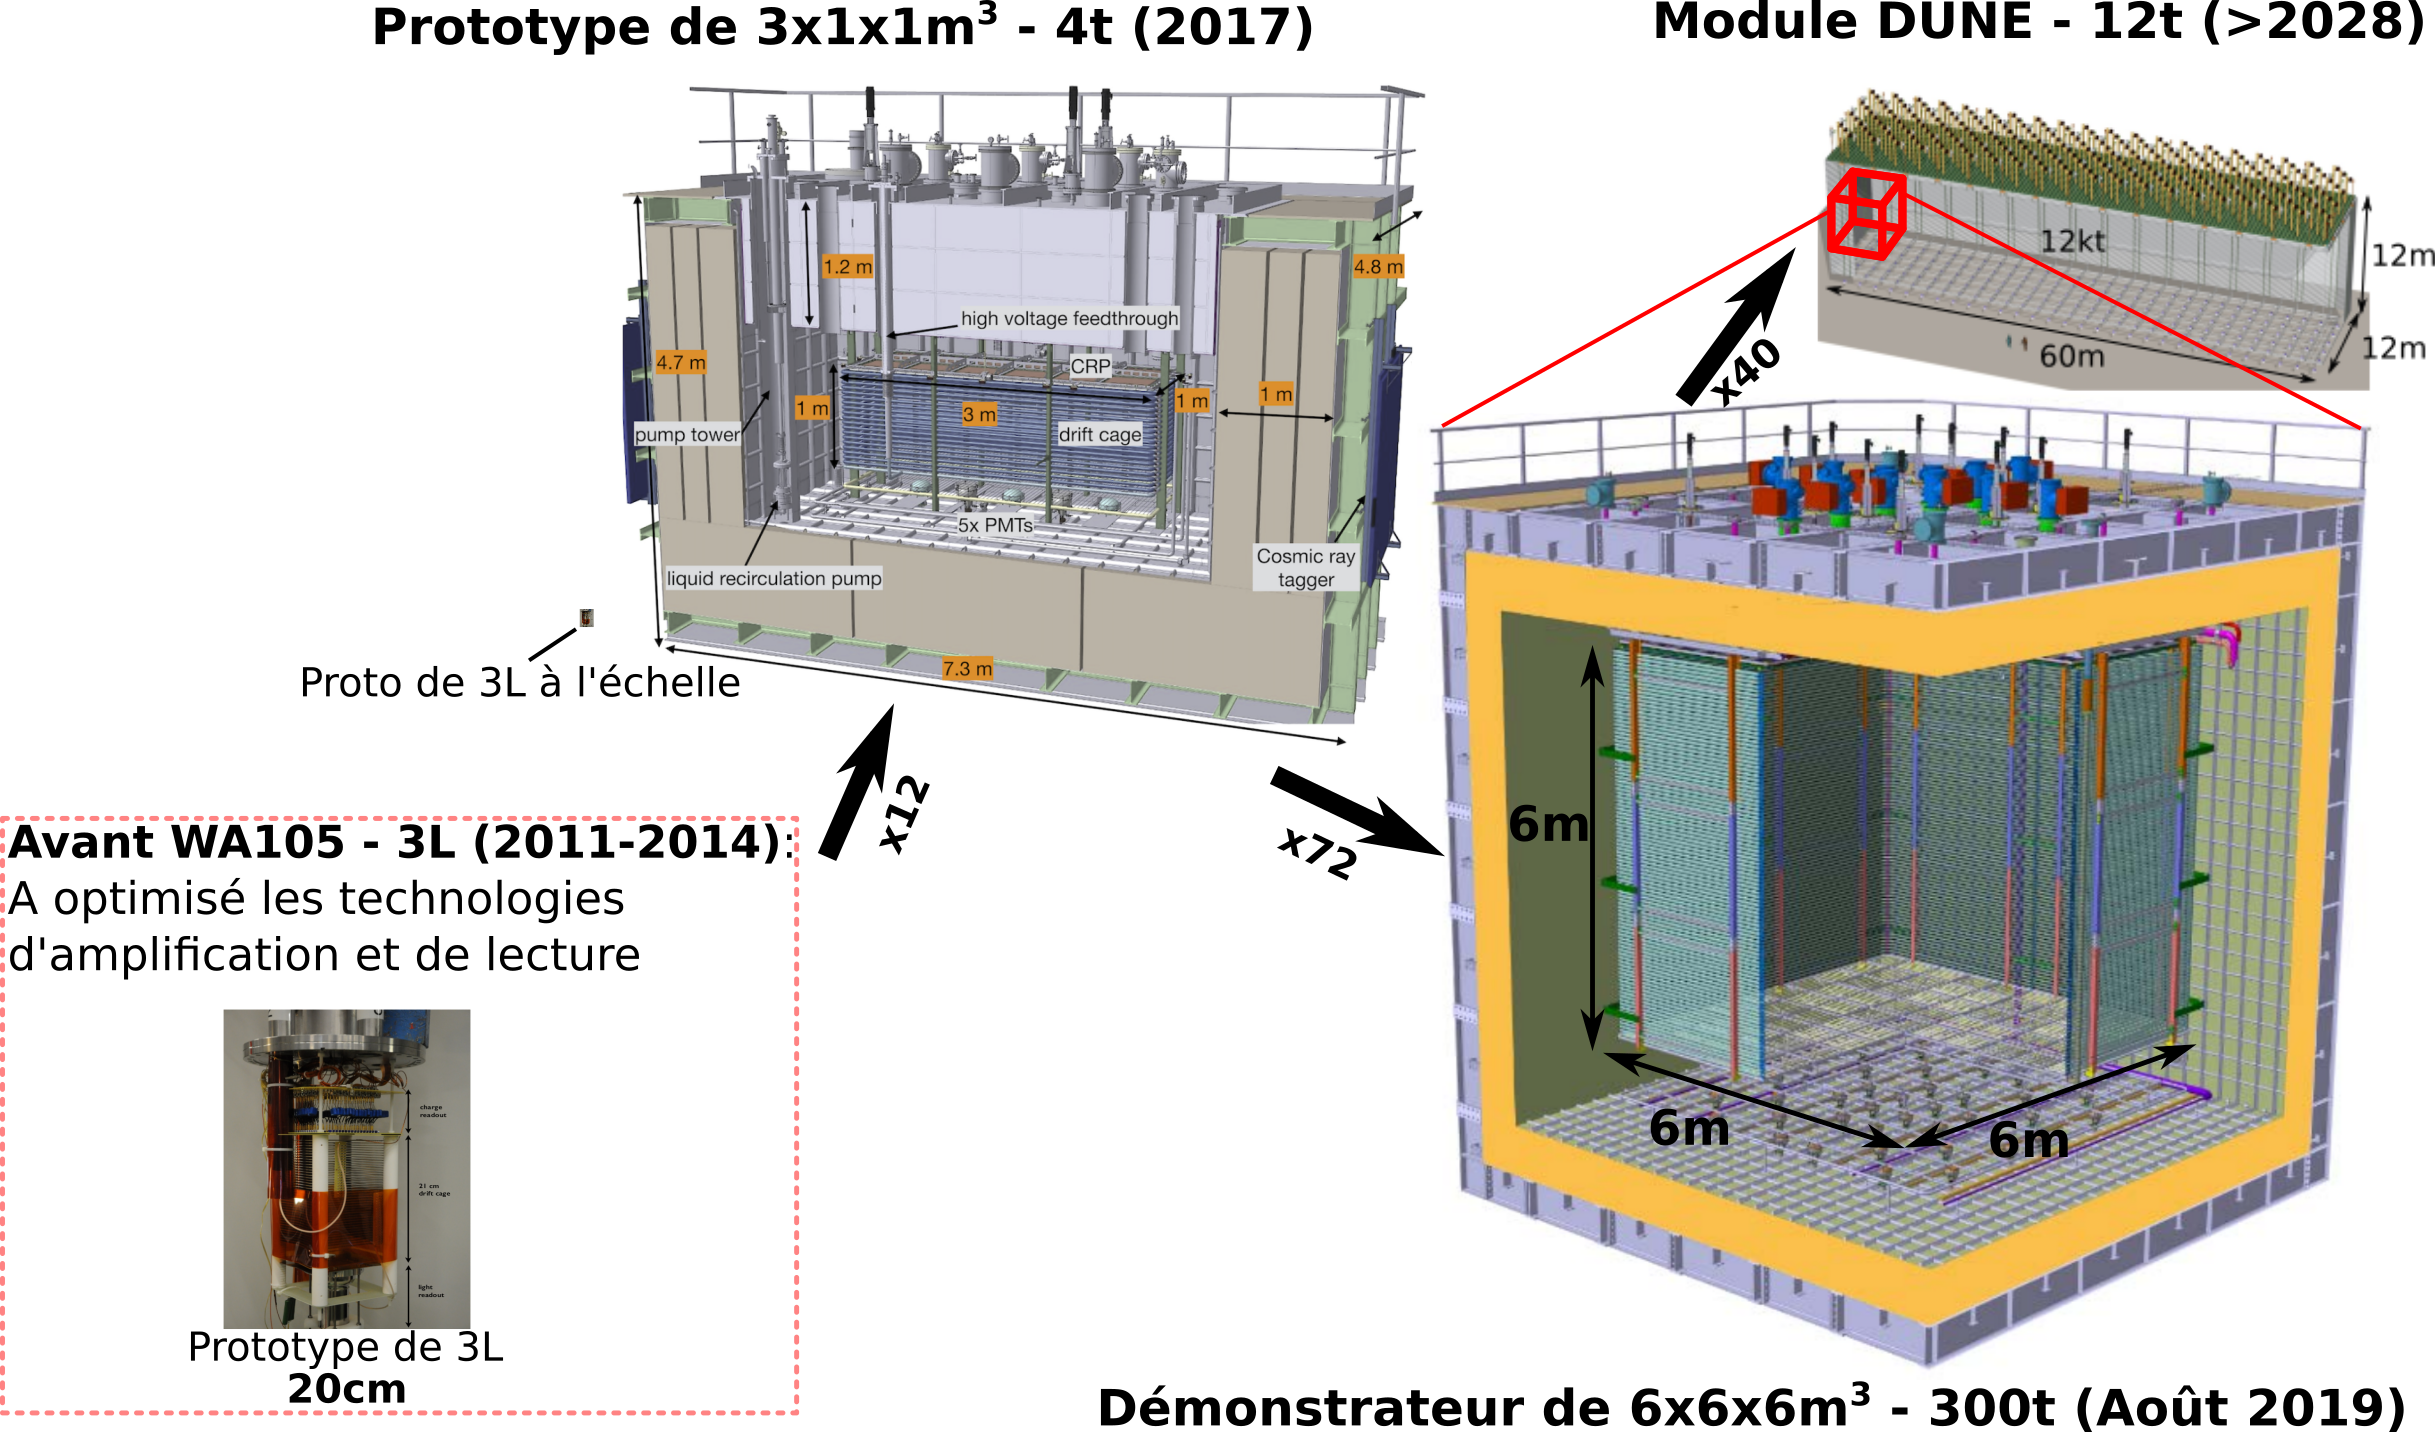
\includegraphics[width=1.03\linewidth]{wa105_scales.png}
    \end{frame}

    \section[Tests des CRPs]{Tests et mesures sur les CRPs du \SSS{}}

    {
    	\usebackgroundtemplate{
\includegraphics[width=\paperwidth]{./pictures/1.pdf}}
        \begin{specialframe}
            \vspace{2cm}\hspace*{-1.8cm}\parbox[t]{\textwidth}{
                \begin{center}
                    \begin{Huge}
                            \textcolor{pheniics_purple}{\textbf{Tests et mesures sur les CRPs du \SSS{}}}
                    \end{Huge}
                \end{center}
            }
        \end{specialframe}
    }

    \begin{frame}{Le démonstrateur de \SSS{}}
    	\begin{scriptsize}
                \centering
    			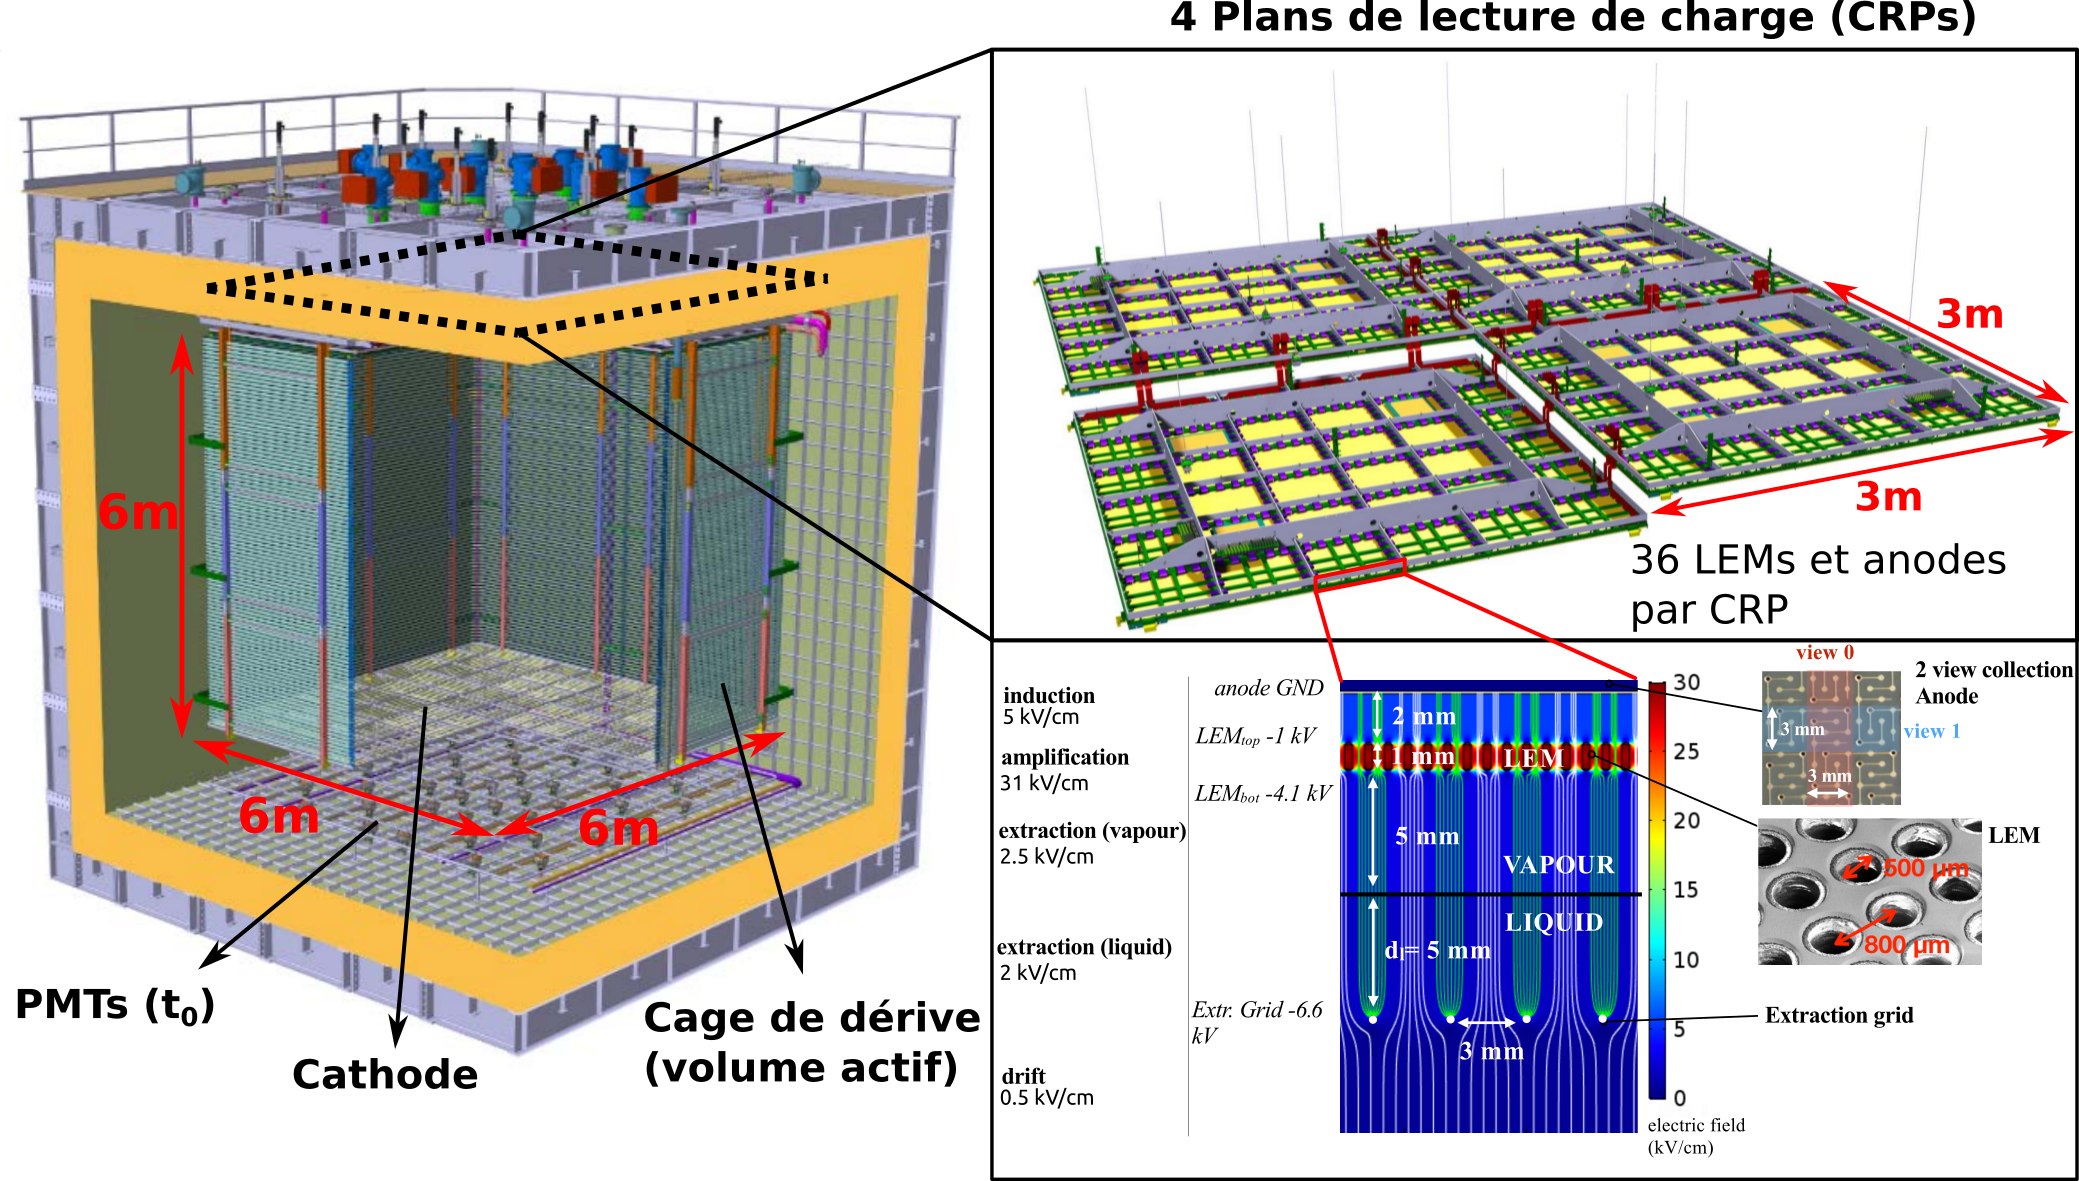
\includegraphics[width=0.9\textwidth]{666_full.png}\\
    			\vfill
    			\textbf{Nouvelle technologie : principaux défis :}\\
    			\begin{minipage}{0.32\textwidth}
    				\begin{itemize}
    					\item[$\bullet$] \textcolor{red}{But: Gain $\geq 20$} \\(S/B $\geq 200$ pour une MIP)
    					\item[$\bullet$] \textcolor{red}{Stabilité sur de très longues périodes (DU$\nu$E $\sim$ 20 ans)}
    				\end{itemize}
    			\end{minipage}\hfill
    			\begin{minipage}{0.32\textwidth}
    				\begin{itemize}
    					\item[$\bullet$] Impuretés: 0.1\;ppb
    					\item[$\bullet$] Effet de charge d'espace
    					(pas dans DU$\nu$E)
    				\end{itemize}
	    		\end{minipage}\hfill
	    		\begin{minipage}{0.32\textwidth}
	    			\begin{itemize}
	    				\item[$\bullet$] Grande distance de dérive (Cathode à \SI{300}{\kilo\volt})
	    				\item[$\bullet$] Extrapolable à l'échelle de DU$\nu$E
	    			\end{itemize}
	    		\end{minipage}
    	\end{scriptsize} 
    \end{frame}

    \begin{frame}{Le sandwich LEM-anode}
	   		\begin{minipage}{0.48\textwidth}
	   			\begin{scriptsize}
		   			\textbf{Gain effectif:}\\
		   		\end{scriptsize}
	   			$G_{eff} = \mathcal{T}e^{A\rho d e^{-B\rho d/V}}$\\
	   			\begin{scriptsize}
	    			\begin{itemize}
	    				\item[$\bullet$] $\mathcal{T}$: Transparence électrique du sandwich LEM-anode.
	    				\item[$\bullet$] $A,B$: coefficients, dépendent du gaz.
	    				\item[$\bullet$] $d$: distance d'amplification (\SI{1}{\milli\meter}).
	    				\item[$\bullet$] $V$: tension d'amplification ($\sim$\SI{3}{\kilo\volt}).
	    				\item[$\bullet$] $\rho$: densité du gaz ($\propto P/T$).
	    			\end{itemize}
	    		\end{scriptsize} 
	   			\vfill
                \centering
				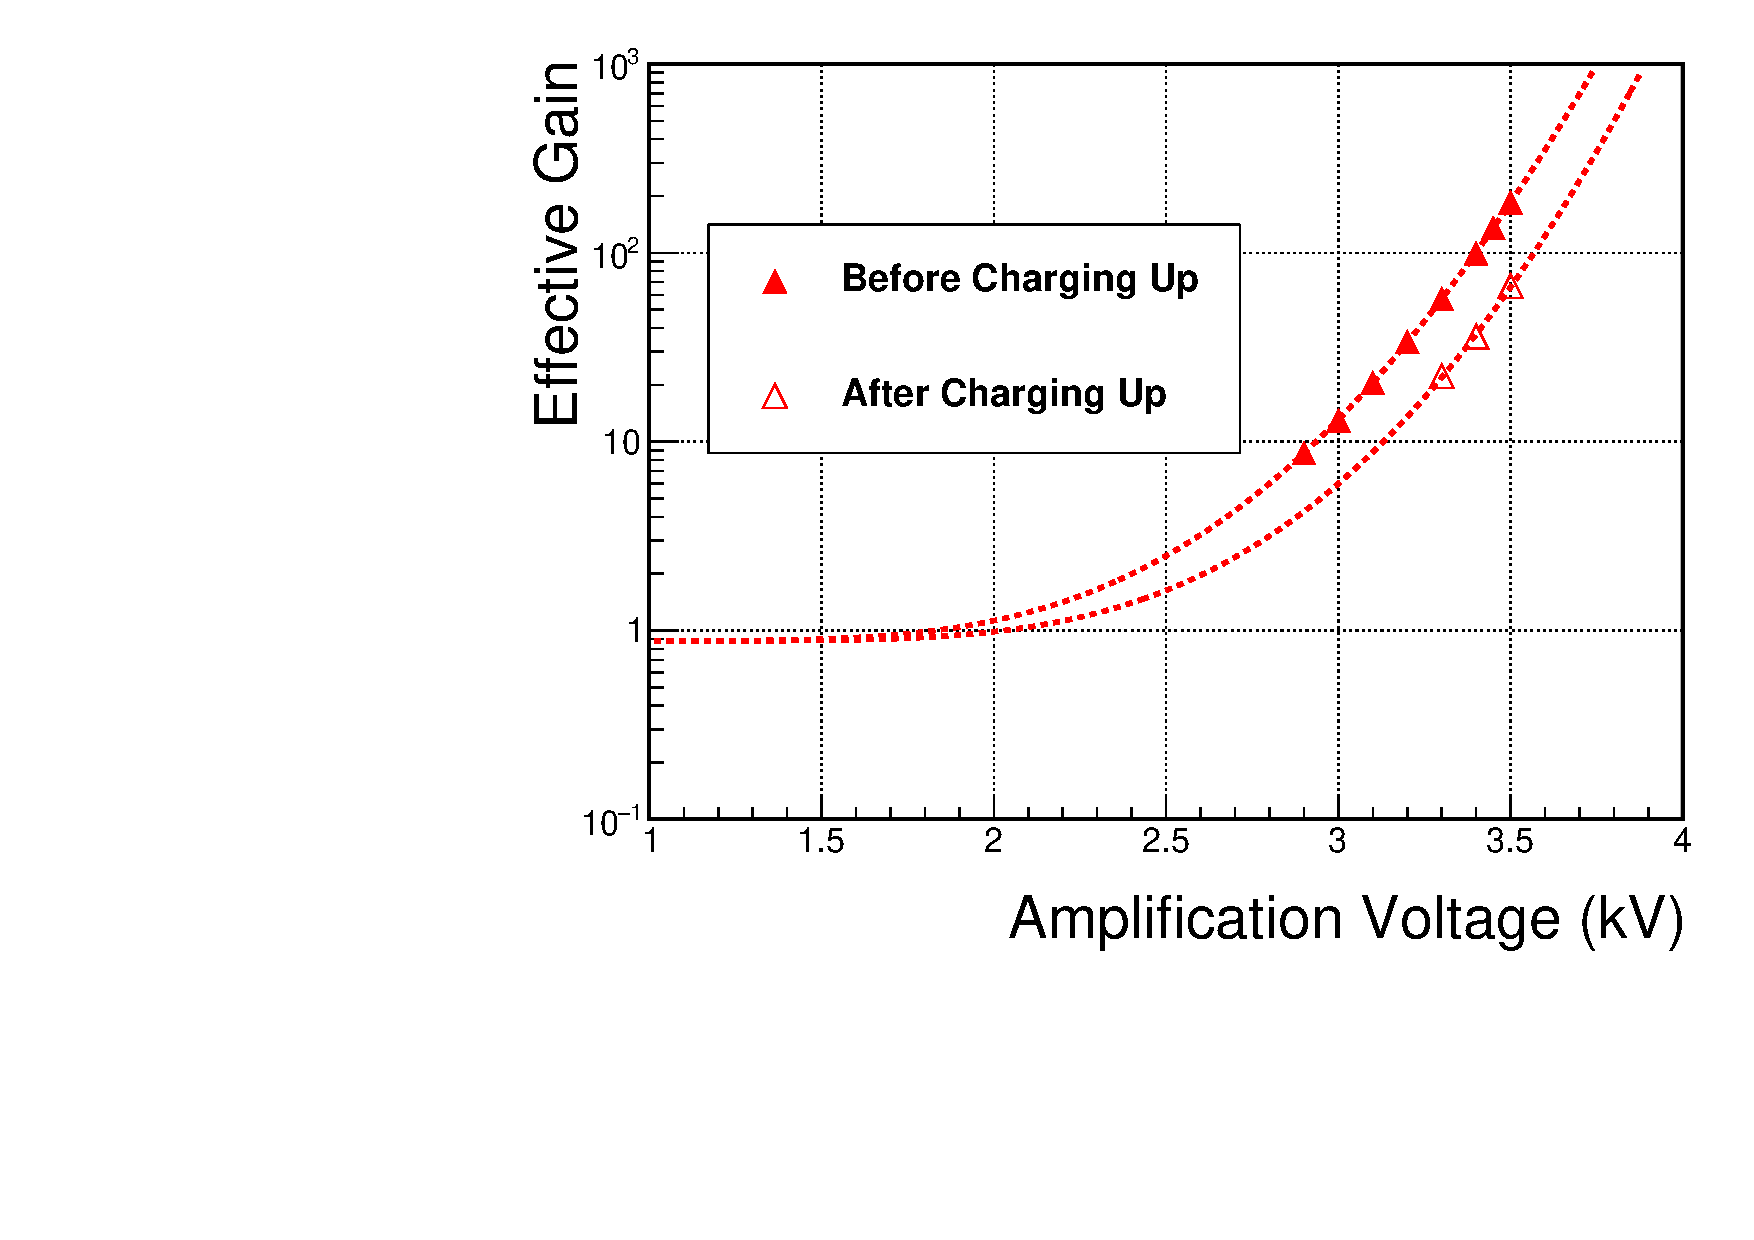
\includegraphics[width=0.8\textwidth]{gain_3L.pdf}
	   		\end{minipage}\hfill
	   		\begin{minipage}{0.48\textwidth}
	   			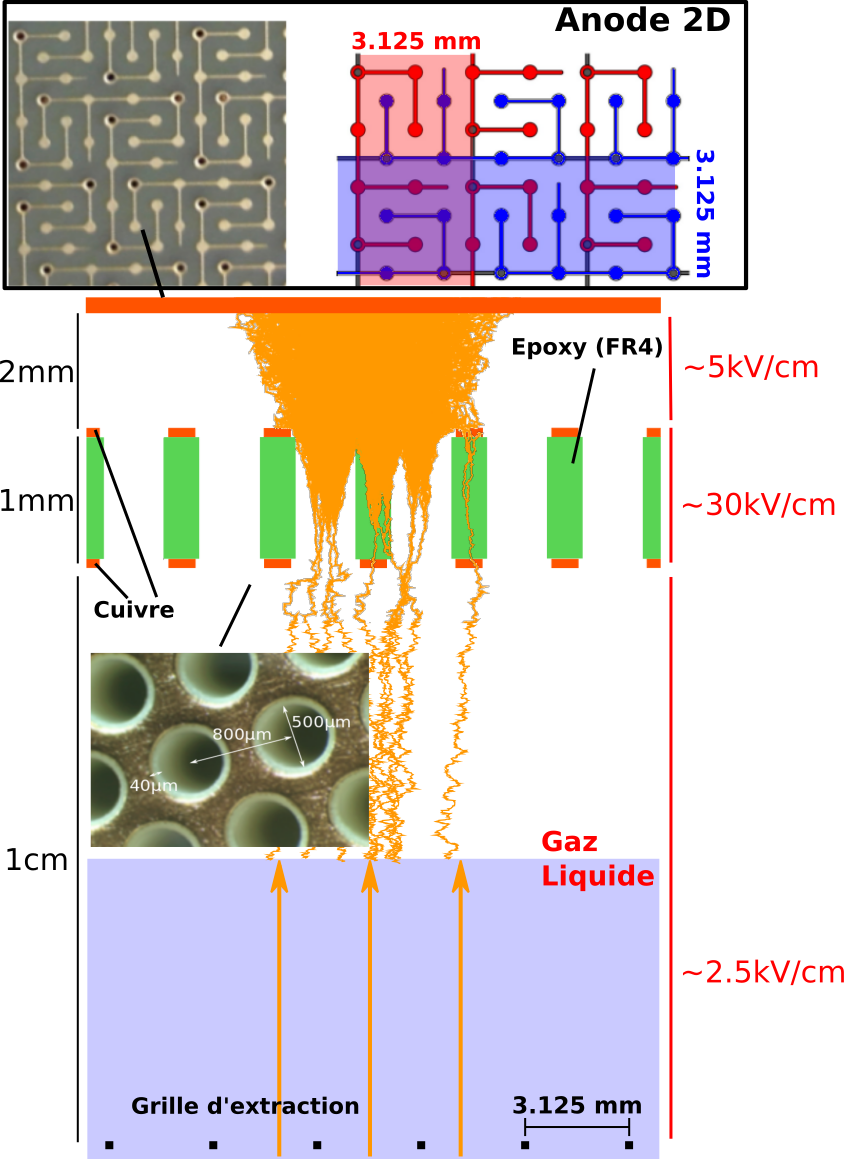
\includegraphics[width=\textwidth]{lem_anode.png}
	   		\end{minipage}
    \end{frame}

    \begin{frame}{La mission de l'Irfu}
    	\begin{scriptsize}
            \textbf{\textcolor{red}{Mission de l'Irfu}: }Tester et caractériser les LEMs et anodes de 2 des 4 CRPs.\\\vfill
		\end{scriptsize}
        Construction infrastructures pour tests LEMs\\
        Production par ELTOS\\
        CFR-34 : été 2017 -> bad -> CFR35 : Jan 2018 -- Oct 2018\\
        2 CRPs intrumentés\\
    \end{frame}

    \begin{frame}{Préparation des LEMs}
    	\begin{scriptsize}
    		\begin{center}
		    	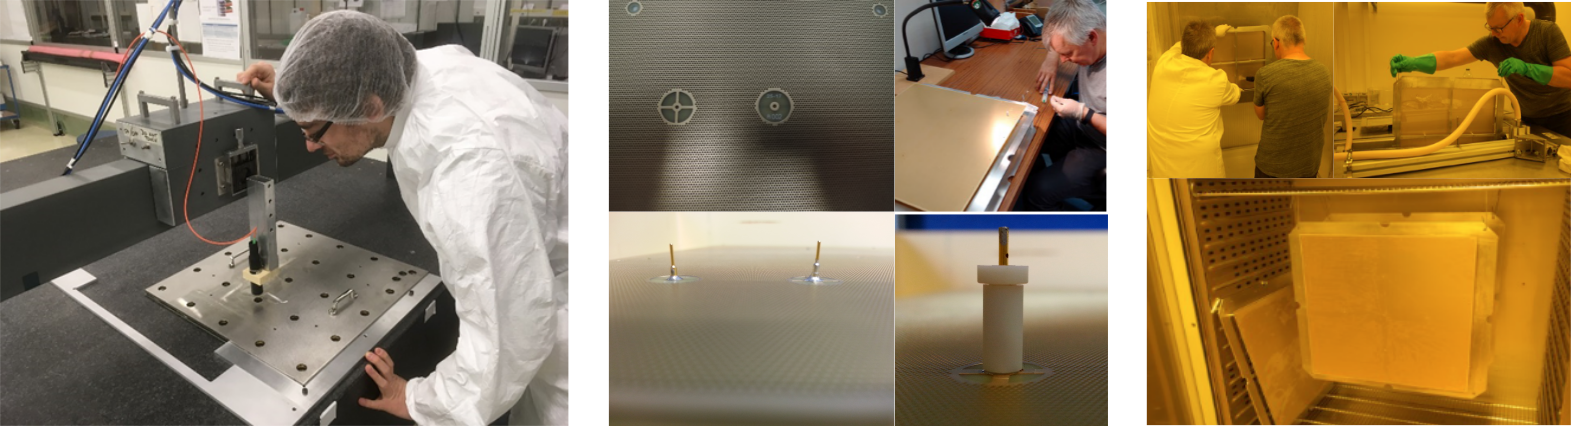
\includegraphics[width=\textwidth]{pretest.png}
	    	\end{center}
	    	\begin{columns}
	    		\begin{column}{0.5\textwidth}
	    			\begin{itemize}
	    				\item[$\bullet$] ELTOS vérifie que les spécifications sont respectées: épaisseurs, RIMs, trous, taille.
	    			\end{itemize}
	    		\end{column}\hfill
	    		\begin{column}{0.5\textwidth}
	    			\textbf{Au DEDIP}:
	    			\begin{itemize}
	    				\item[$\bullet$] Mesure de l'épaisseur.
	    				\item[$\bullet$] Soudure des connecteurs haute tension, collage des séparateurs MACOR.
	    				\item[$\bullet$] Nettoyage, polymérisation, séchage.
	    			\end{itemize}
	    		\end{column}
	    	\end{columns}
	    \end{scriptsize}
        $\Rightarrow$ LEM près pour les tests hautes tensions et mesures de gain!
    \end{frame}

    \subsection[Épaisseur]{Mesure de l'épaisseur des LEMs}

     \begin{frame}{Mesure de l'épaisseur des LEMs}{Méthode expérimentale}
    	\begin{scriptsize}
    		\begin{columns}
    			\begin{column}{0.5\textwidth}
    				\begin{center}
    					$G _{eff}= \mathcal{T}e^{A\rho \textcolor{red}{d} e^{-B\rho \textcolor{red}{d}/V}}$\\
    				\end{center}
    				$\textcolor{red}{d}$: Distance d'amplification, i.e \textcolor{red}{épaisseur du LEM}.\\
    				$\Rightarrow$ Impact exponentiel sur le gain.\\
    				$\Rightarrow$ Nécessaire de connaître les fluctuations de cette épaisseur pour \textcolor{red}{vérifier l'uniformité du gain}.\\
    				\vfill
    				\centering 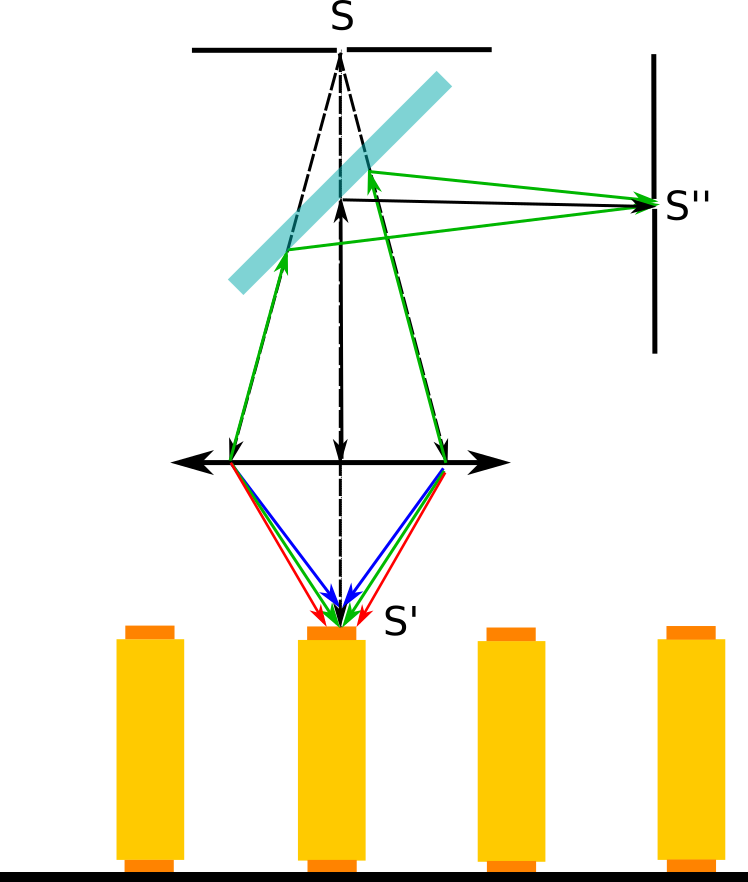
\includegraphics[height=0.6\textheight]{CCI.png}\\\vfill
    			\end{column}
    			\hfill
    			\begin{column}{0.5\textwidth}
    				\begin{itemize}
    					\item[$\bullet$] Utilise Imagerie Chromatique Confocal.
    					\item[$\bullet$] Mesure l'épaisseur des 72 LEMs du \SSS{}.
    					\item[$\bullet$] Création d'un script Python pour l'analyse des résultats.
    				\end{itemize}
    				\centering 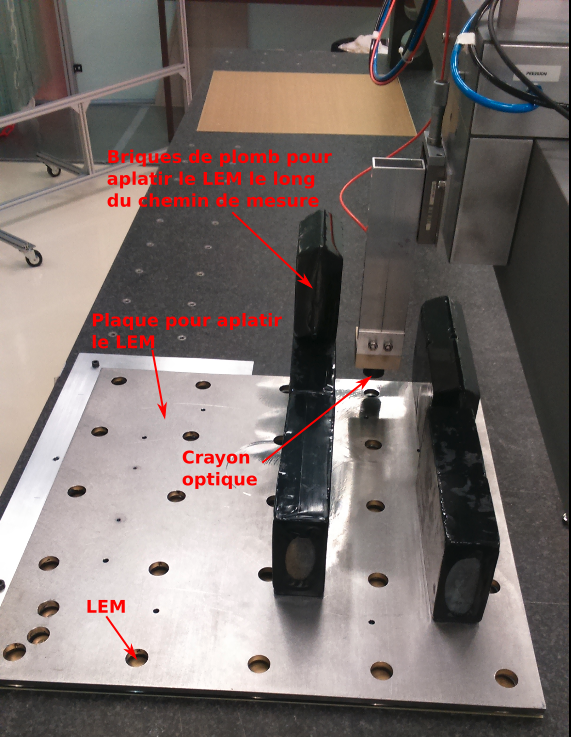
\includegraphics[height=0.6\textheight]{./pictures/plate_and_bricks.png}\\
    			\end{column}
    		\end{columns}
    	\end{scriptsize}
    \end{frame}

    \begin{frame}{Mesure de l'épaisseur des LEMs}{Résultats}
    	\begin{scriptsize}
    		\begin{columns}
    			\begin{column}{0.48\textwidth}
    				\centering
    				Épaisseur dans un trou de mesure\\
    				\centering
    				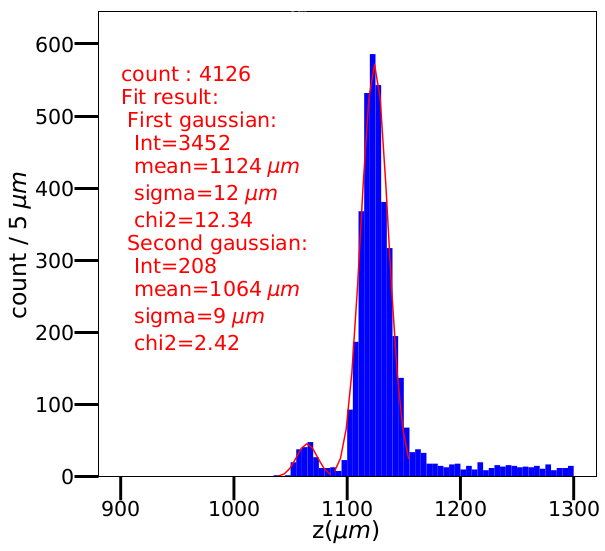
\includegraphics[width=0.7\textwidth]{distri_1_trou_lem.png}\\
    				\vspace{0.15cm}
    				\centering
    				Épaisseur moyenne (36 LEMs)\\
    				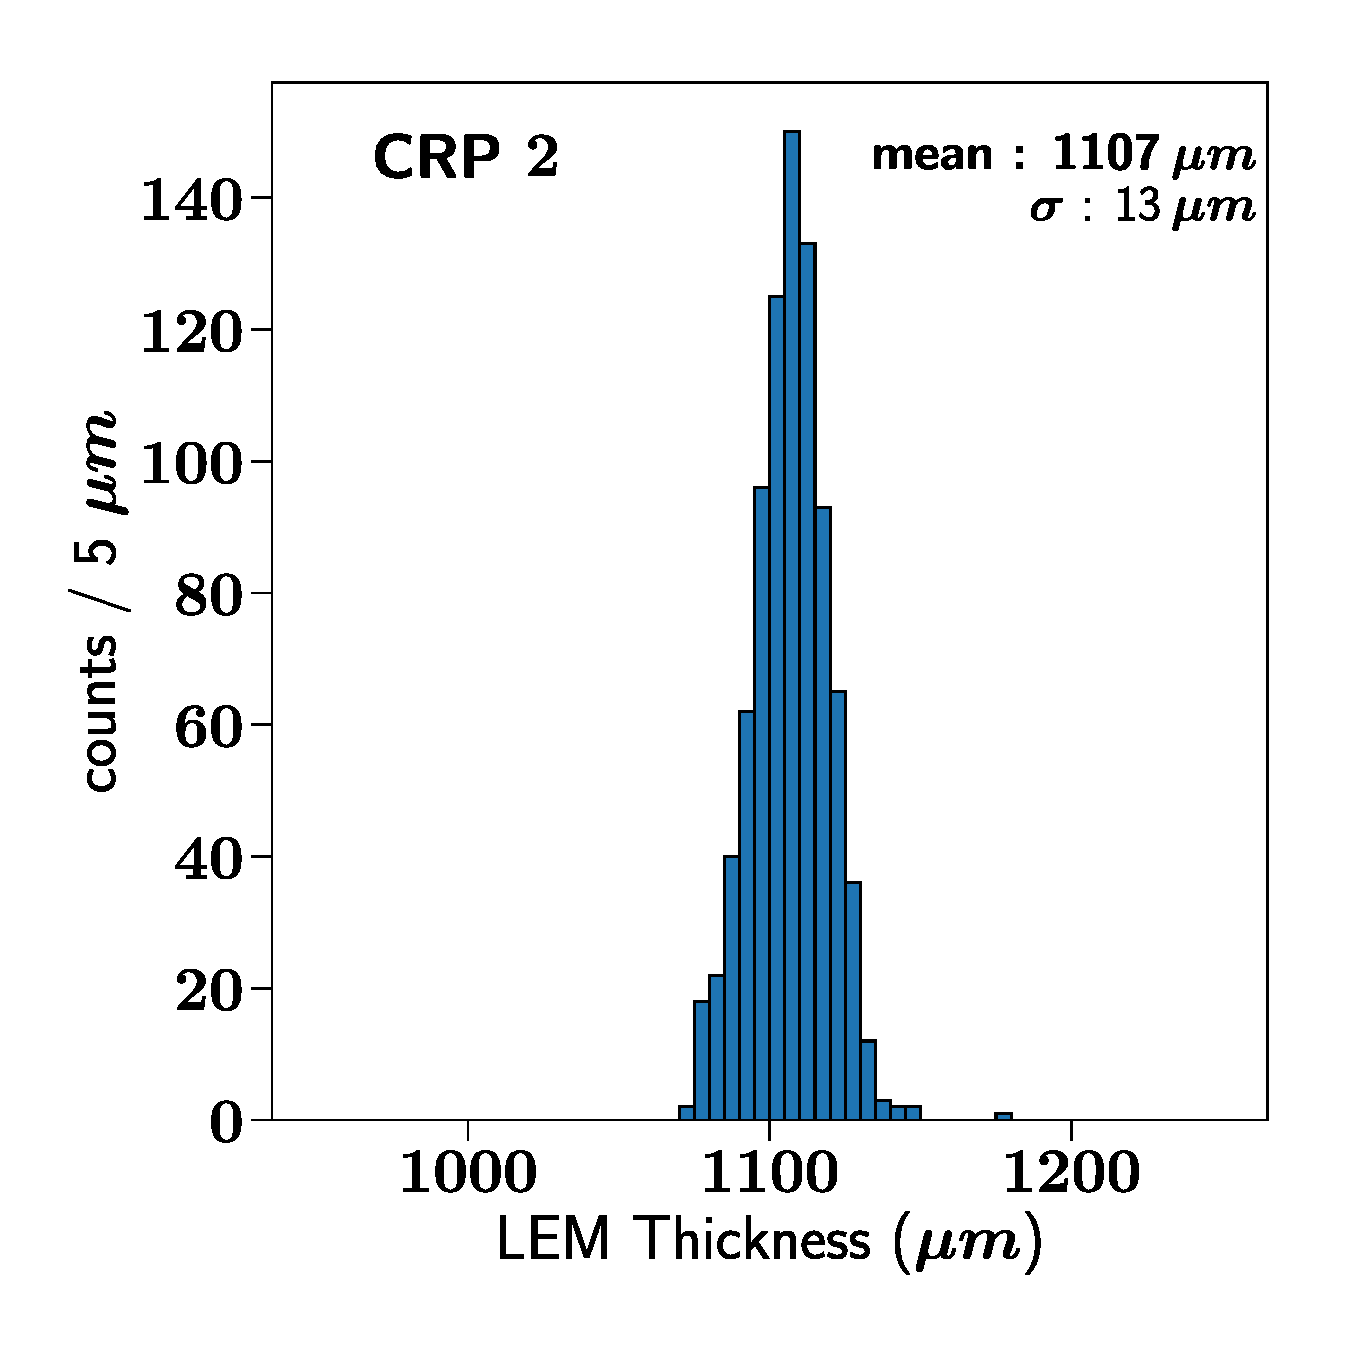
\includegraphics[width=0.7\textwidth]{LEM_sum_all_histo_CERN.pdf}
    			\end{column}
    			\hfill
    			\begin{column}{0.48\textwidth}
    				\centering
    				Uniformité de l'épaisseur dans 1 LEM\\
    				\centering
    				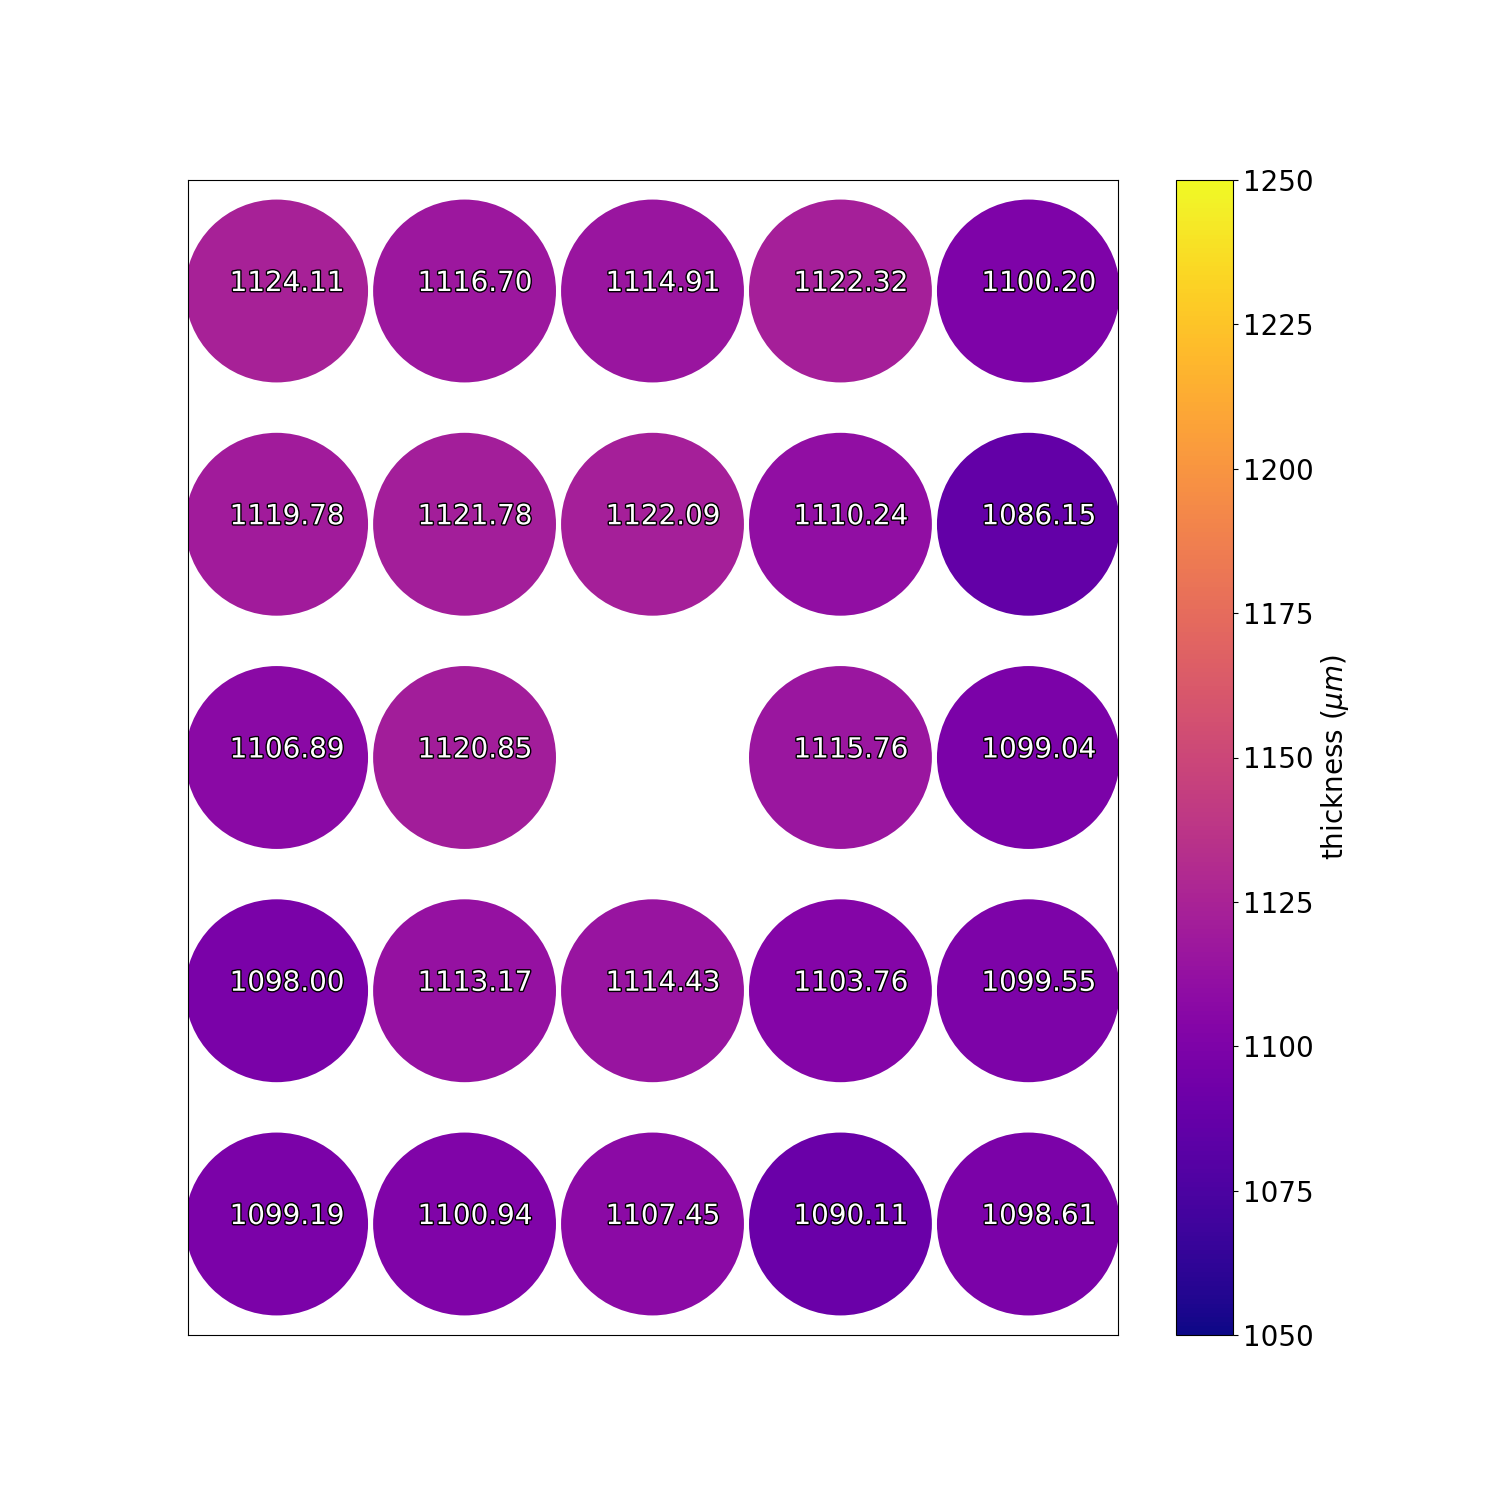
\includegraphics[width=0.6\textwidth]{2D_LEM_thickness_distri.png}\\
    				\vspace{0.15cm}
    				\centering
    				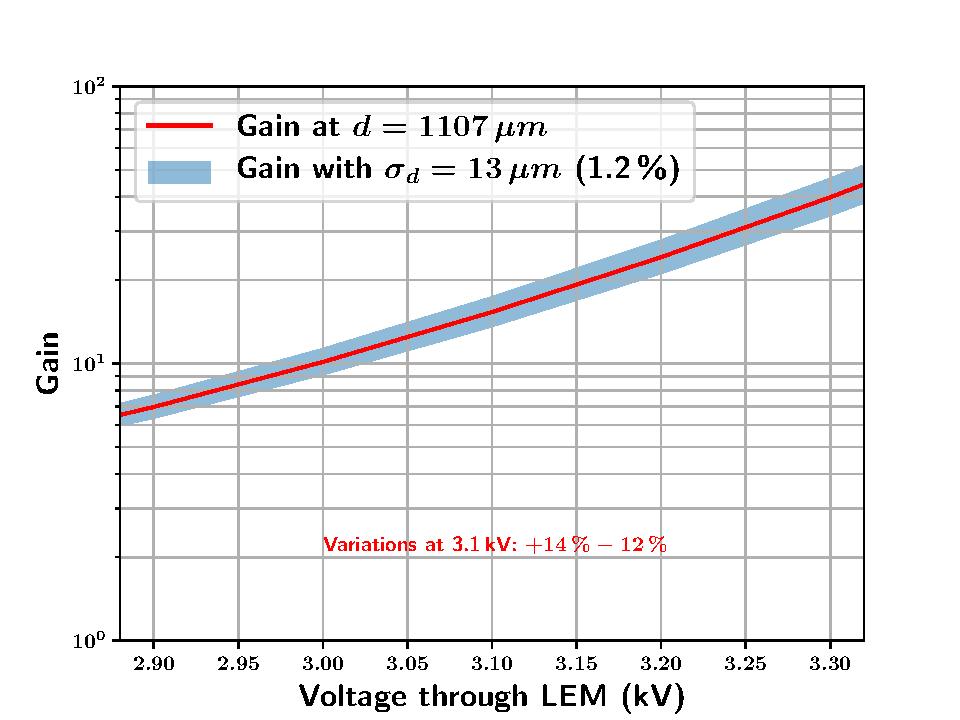
\includegraphics[width=\textwidth]{measured_gain_fluctuations.pdf}
    			\end{column}
    		\end{columns}
    	\end{scriptsize}
    \end{frame}

%  \begin{frame}{frame title}{frame subtitle}
%      \begin{block}{LEMs}
%        \begin{columns}
%          \column{.5\textwidth} \hspace{0.5cm}
%          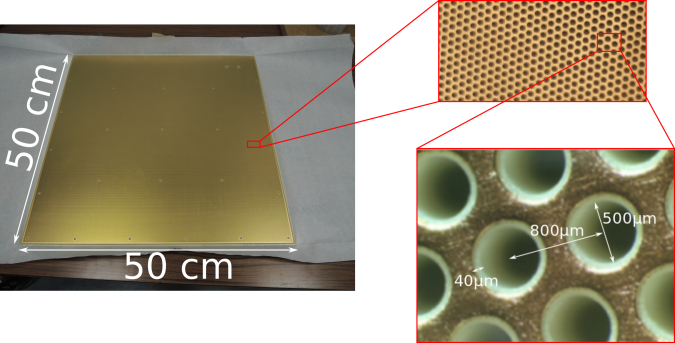
\includegraphics[width=0.7\textwidth]{LEM_zoom.png} 
%          \column{.5\textwidth}
%          \textit{text}
%        \end{columns}
%      \end{block}
%      \pause
%      \begin{block}{Anodes}
%        \begin{columns}
%          \column{.5\textwidth} \hspace{0.5cm}
%          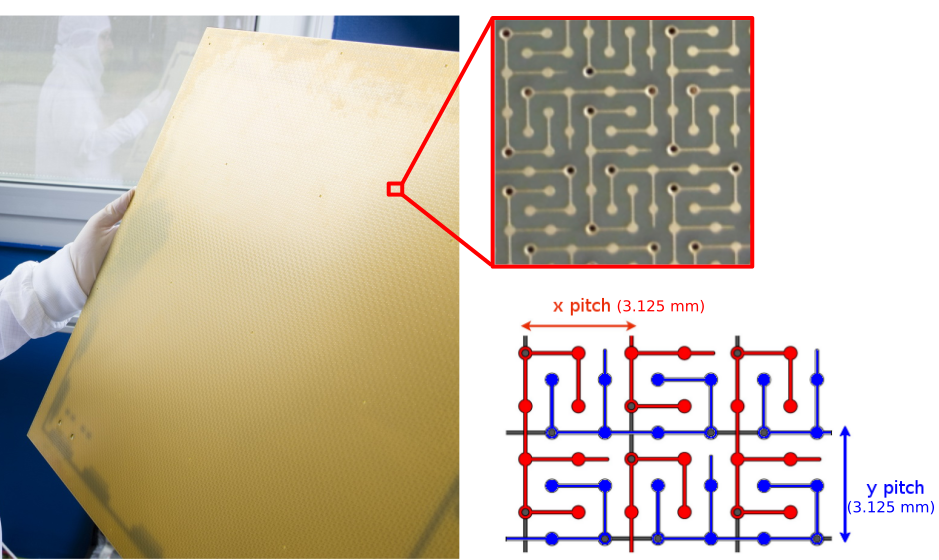
\includegraphics[width=0.7\textwidth]{anode.png} 
%          \column{.5\textwidth}
%          \textit{Text}
%        \end{columns}
%      \end{block}
%  \end{frame}


    \subsection[Tension et gain]{Tenue en tension et gain des LEMs}

    \begin{frame}{Tenue en tension des LEMs}
    	\begin{scriptsize}
    		\begin{center}
    			\textbf{Teste des LEMs à la desité d'une DLArTPC dans une enceinte haute pression : Haute tension maximum}\\
    			$G _{eff}= \mathcal{T}e^{A\textcolor{red}{\rho} d e^{-B\textcolor{red}{\rho}d/\textcolor{red}{V}}}$
    		\end{center} 
    		\begin{columns}
		    	\begin{column}{0.5\textwidth}
		    		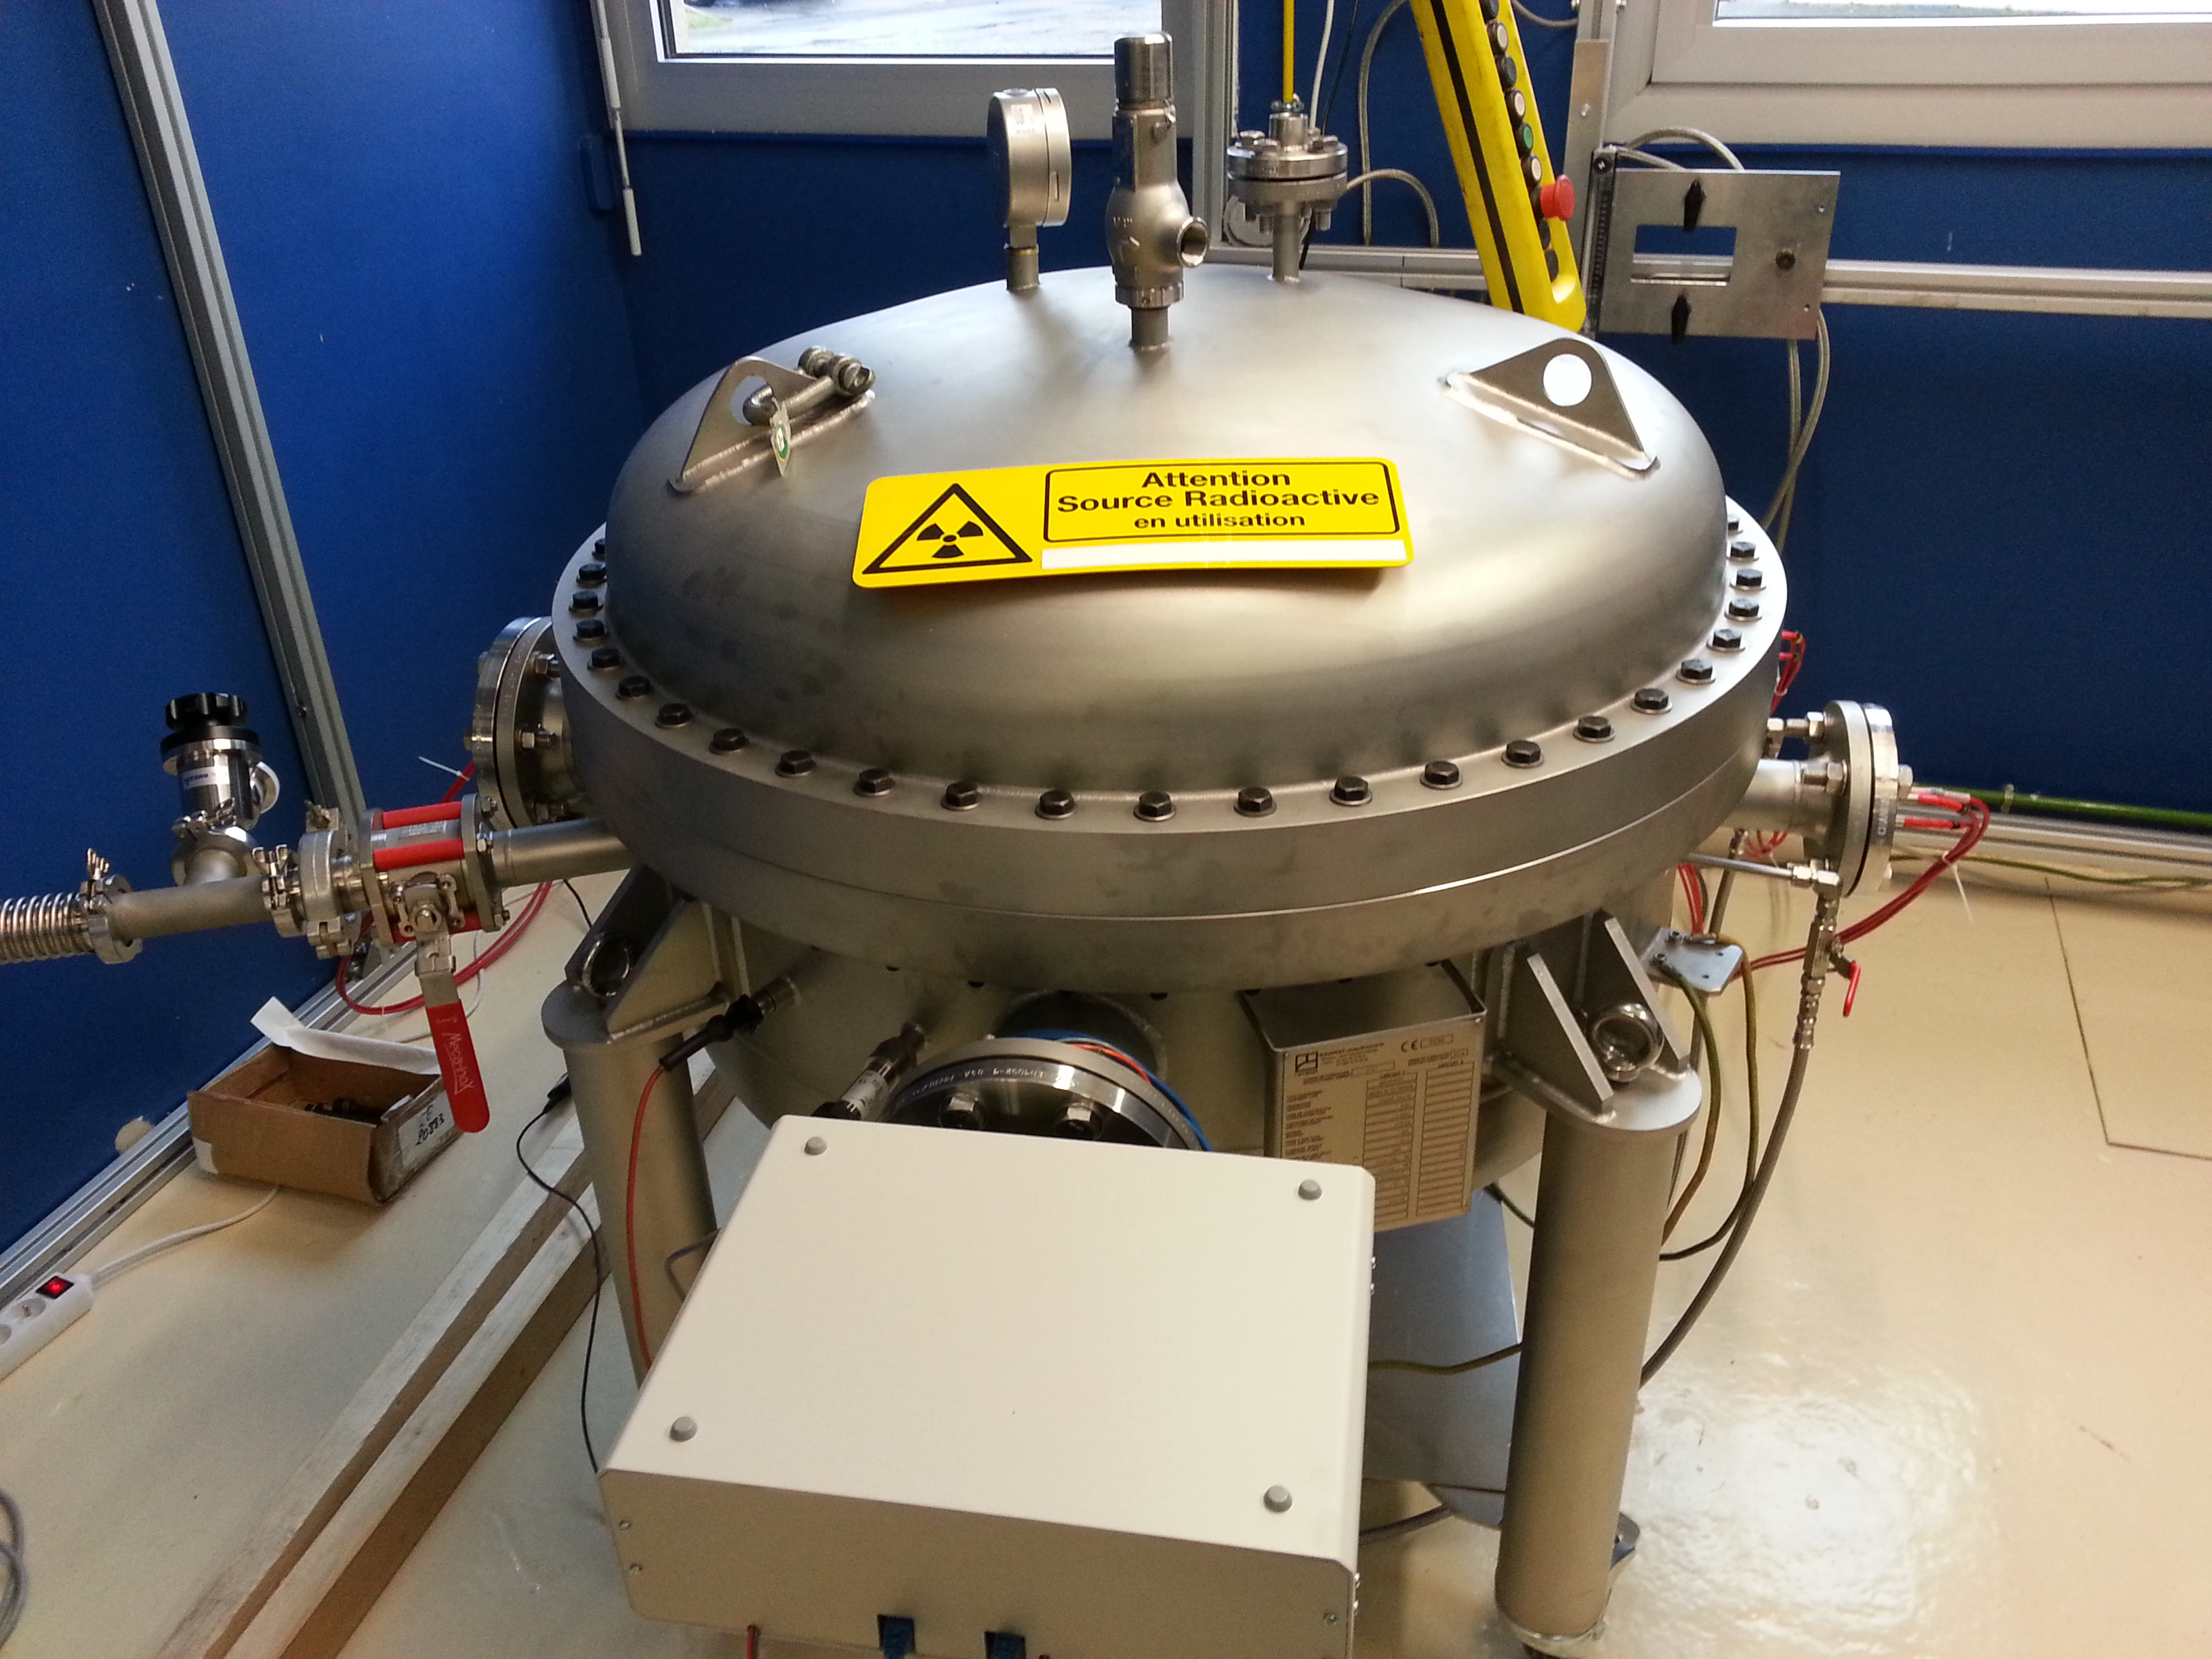
\includegraphics[height=3.7cm]{gamelle.jpg}\\
		    		\begin{itemize}
		    			\item[$\bullet$] $\rho \propto P/T$
		    			\item[$\bullet$] Pas de système cryo : \textcolor{red}{température ambiante}.
		    			\item[$\bullet$] Densité d'une DLArTPC à \textcolor{red}{\SI{3.3}{\bar}}.
		    		\end{itemize}
		    	\end{column}\hfill
		    	\begin{column}{0.5\textwidth}
		    		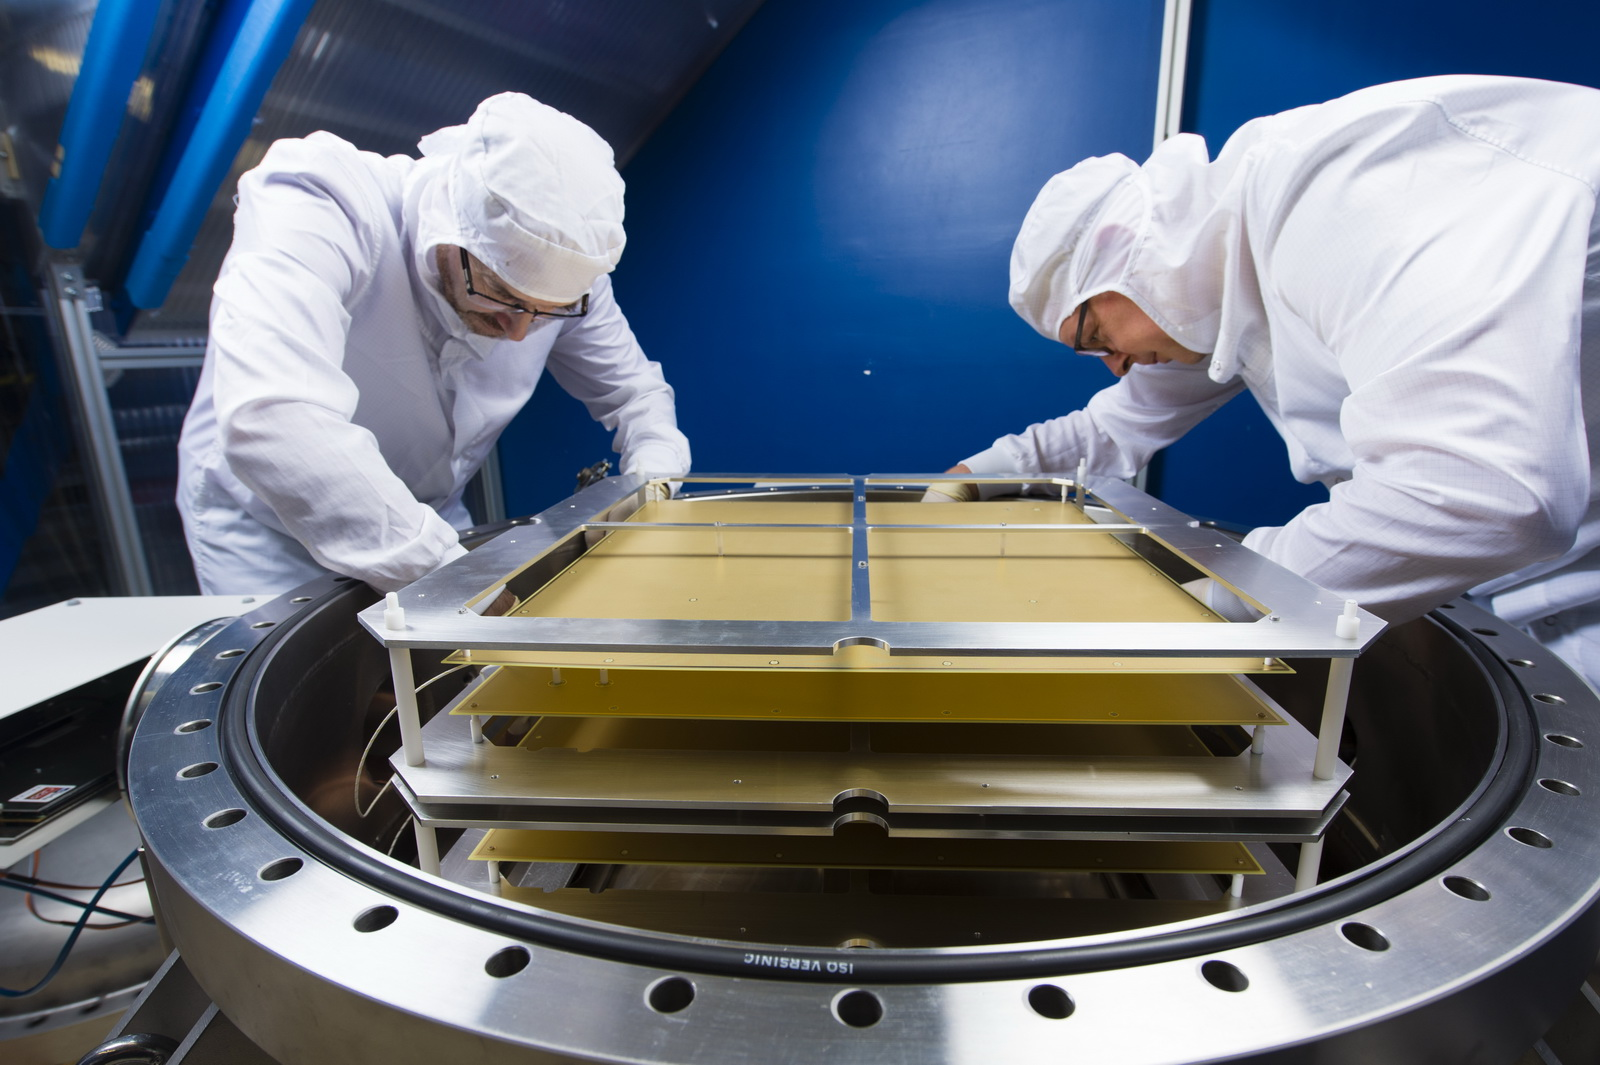
\includegraphics[height=3.7cm]{6lems_gamelle.jpg}\\
		    		\begin{itemize}
		    			\item[$\bullet$] Enceinte haute pressions: remplie d'argon gazeux.
		    			\item[$\bullet$] Empilement de 6-9 LEMs.
		    			\item[$\bullet$] A testé plus de 100 LEMs.
		    		\end{itemize}
		    	\end{column}
		    \end{columns}
	    \end{scriptsize} 
    \end{frame}

    \begin{frame}{Tenue en tension des LEMs}
   		\begin{columns}
    		\begin{column}{0.5\textwidth}
    			\begin{center}
	    			\begin{scriptsize}
		    			CFR-34 à 33--\SI{35}{\kilo\volt\per\centi\meter}\\
		    			\textcolor{red}{$\sim$ 20 décharges par heure}\\
		    		\end{scriptsize}
	    			\begin{tiny}
		    			(Design fait par \textbf{ETHZ}, utilisé dans le \TOO{})
		    		\end{tiny}\\
	    			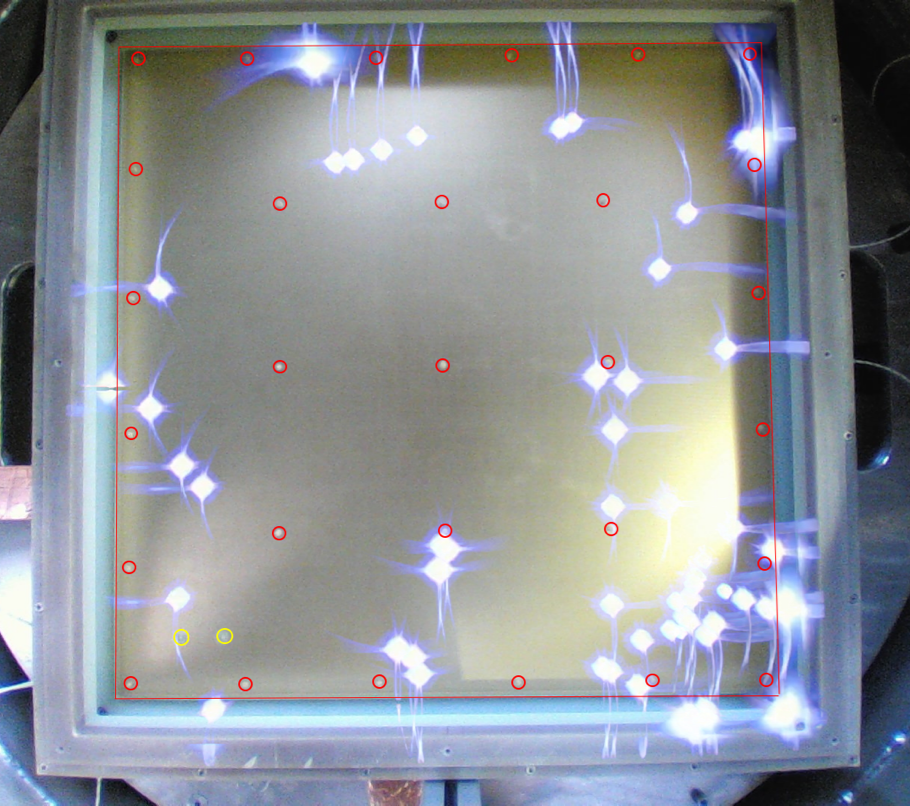
\includegraphics[height=3.1cm]{sparks_34.png}
    			\end{center}
    		\end{column}\hfill
    		\begin{column}{0.5\textwidth}
    			\begin{center}
	    			\begin{scriptsize}
		    			CFR-35 à \SI{35}{\kilo\volt\per\centi\meter} \\
		    			\textcolor{red}{$\sim$ 3 20 décharges par heure}\\
		    		\end{scriptsize}
	    			\begin{tiny}
	    				(Design fait par le \textbf{CEA}, utilisé dans le \SSS{})
	   				\end{tiny}\\
	    			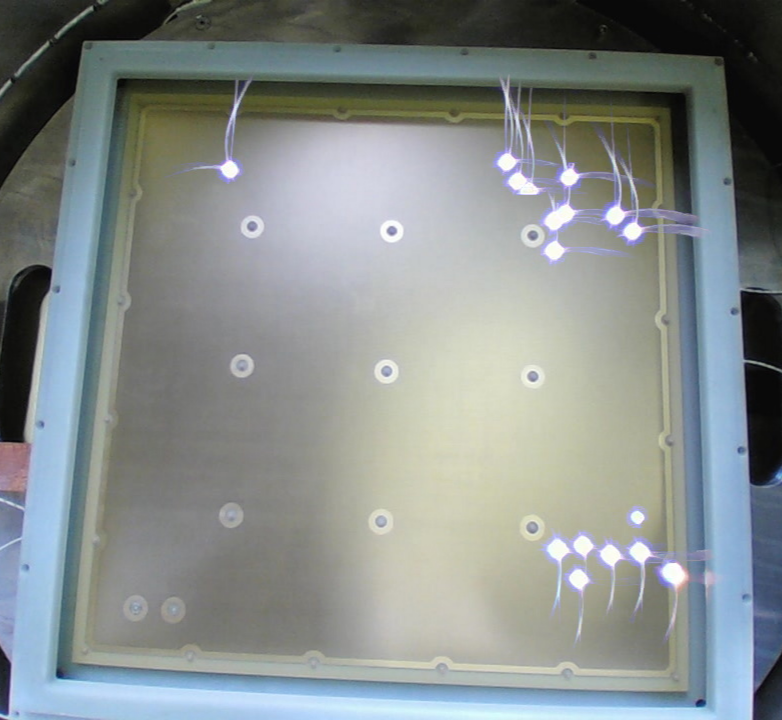
\includegraphics[height=3.1cm]{sparks_35.png}
	    		\end{center}
    		\end{column}
    	\end{columns}\vspace{0.1cm}
    	\begin{columns}
    		\begin{column}{0.5\textwidth}
    			\begin{scriptsize}
	    			\begin{itemize}
	    				\item[$\bullet$] CFR-34 instable au delà de \SI{32}{\kilo\volt\per\centi\meter}.
	    				\item[$\bullet$] Décharges surtout sur les bords et les coins.
	    			\end{itemize}
	    			\begin{itemize}
	    				\item[$\Rightarrow$] Nouveau design (CFR-35) avec bords plus grands.
	    				\item[$\Rightarrow$] Nombre de décharges plus faible d'un ordre de grandeur.
	    			\end{itemize}
	    		\end{scriptsize}
    		\end{column}\hfill
    		\begin{column}{0.5\textwidth}
    			\begin{minipage}{0.48\textwidth}
    				\centering
    				\begin{scriptsize}
	    				CFR-34
	    			\end{scriptsize}
    				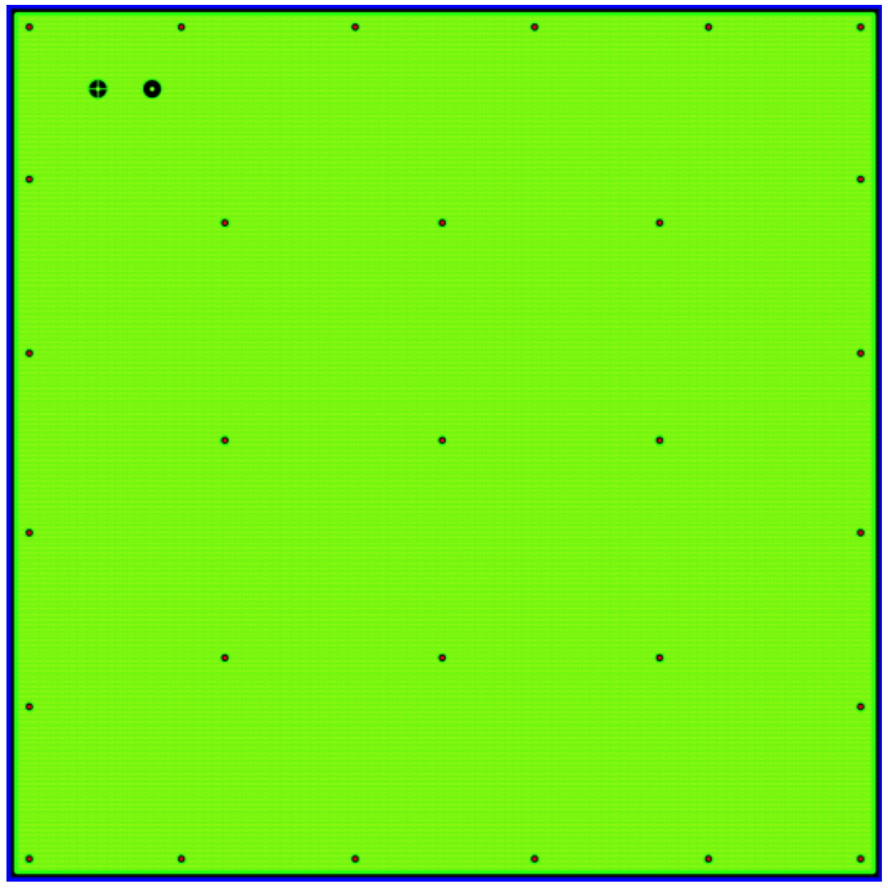
\includegraphics[width=.9\textwidth]{CFR-34.png}
    			\end{minipage}\hfill
    			\begin{minipage}{0.48\textwidth}
    				\centering
    				\begin{scriptsize}
	    				CFR-35
    				\end{scriptsize}
    				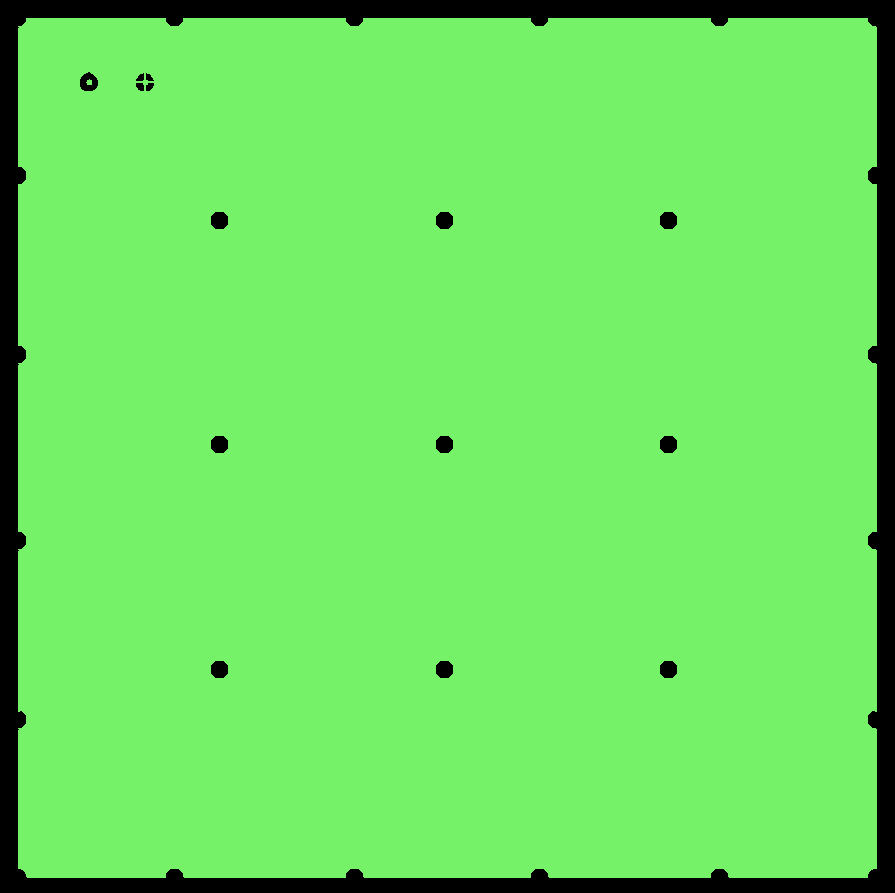
\includegraphics[width=.9\textwidth]{CFR-35.png}
    			\end{minipage}
    		\end{column}
    	\end{columns}
    \end{frame}

    \begin{frame}{Mesures de gain}
        %TODO mettre à jour
    	\begin{scriptsize}
    		\begin{center}\textbf{Teste des LEMs à la desité d'une DLArTPC dans une enceinte haute pression : gain}\\\end{center}
    		\begin{columns}
    			\begin{column}{0.46\textwidth}
    				\centering 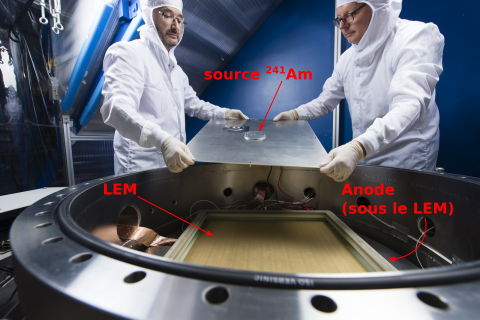
\includegraphics[width=\textwidth]{gamelle_source.png}
    			\end{column}\hfill
    			\begin{column}{0.58\textwidth}
    				\centering 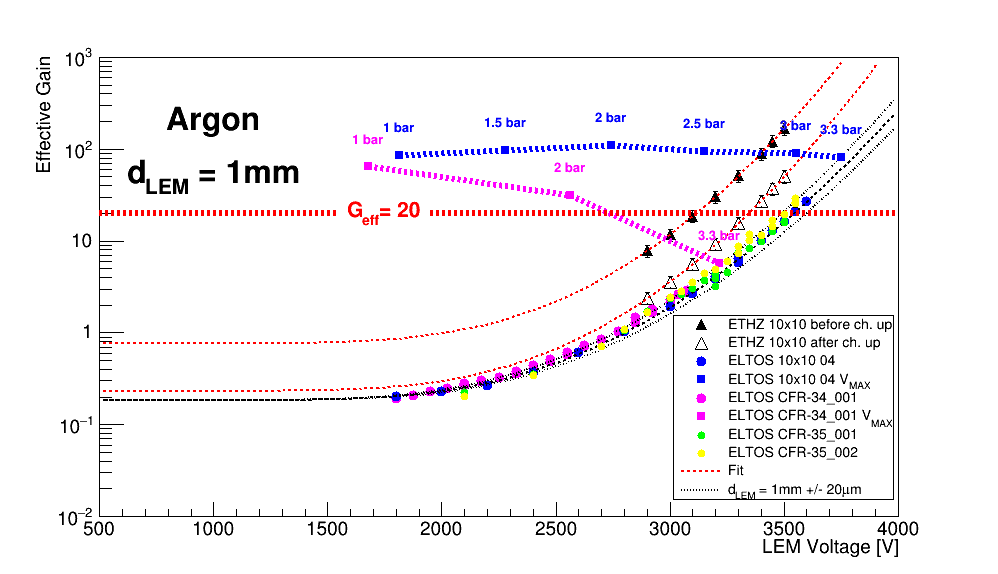
\includegraphics[width=\textwidth]{./pictures/gain.png}
    			\end{column}
    		\end{columns}\vfill
    		\begin{columns}
    			\begin{column}{0.38\textwidth}
    				\begin{itemize}
    					\item[$\bullet$] 1 sandwich LEM-anode.
    					\item[$\bullet$] Source $^{241}$Am.
    					\item[$\bullet$] Peut mesurer le gain.
    				\end{itemize}
    			\end{column}\hfill
    			\begin{column}{0.58\textwidth}
    				\begin{itemize}
    					\item[$\bullet$] Gain dans les LEMs de $10\times$\SI{10}{\centi\meter\squared} et $50\times$\SI{50}{\centi\meter\squared} se comporte de la même manière
    				\end{itemize}
    			\end{column}
    		\end{columns}
%    		\vfill
%    		\textbf{$\Rightarrow$ Use CFR-35 for $\mathbf{6 \boldsymbol{\times} 6 \boldsymbol{\times} \SI[detect-weight]{6}{\meter\cubed}}$}.\\
    		%\textbf{Note:} Not sure about absolute gain value. Based on 3L measurements, CFR-35 should reach gain of $\sim$200.
    	\end{scriptsize}
    \end{frame}

{
	\setlength\pdfpagewidth{12.8cm}%
	\setlength\pdfpageheight{9cm}%
	\usebackgroundtemplate{\includegraphics[width=\paperwidth]{CRP_bottom.png}}
	\begin{frame}[plain]
	\end{frame}
}

    \begin{frame}{Boîte cryogénique au CERN}
    	%the planarity obtained is within 1.2 mm over the entire plane (mail Dominique 21/09/2018)
        %TODO : rajouter discussion à propos des variations induites pas la planéité
   		\begin{columns}
   			\begin{column}{0.4\textwidth}
   				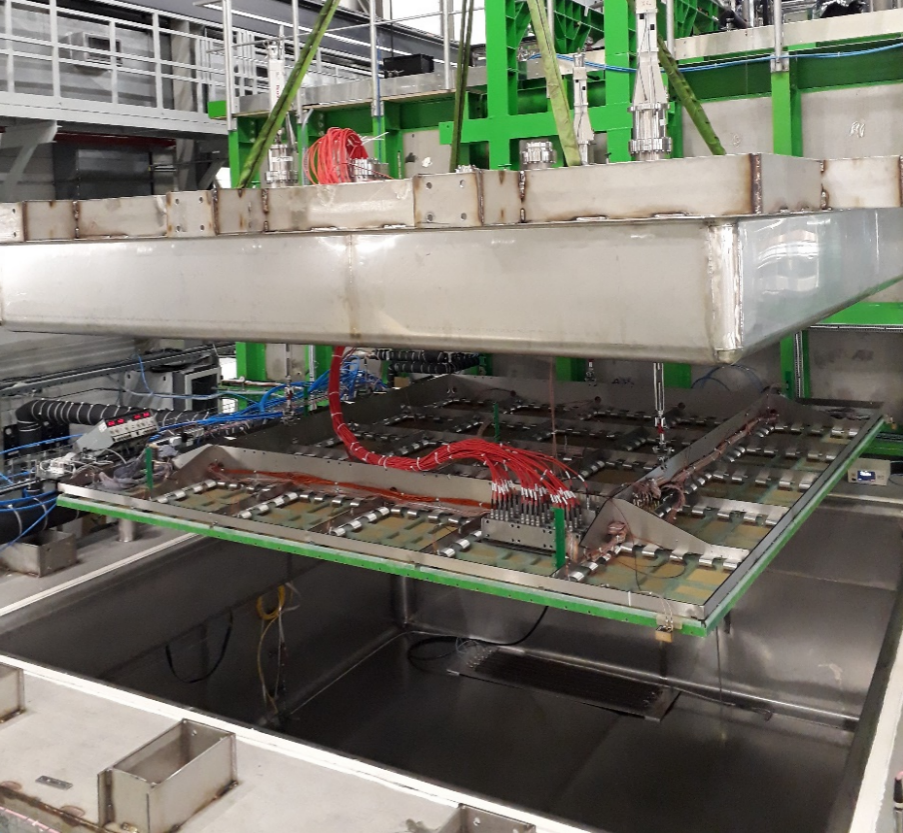
\includegraphics[width=\textwidth]{./pictures/crp_inserting_coldbox.png}\\
   				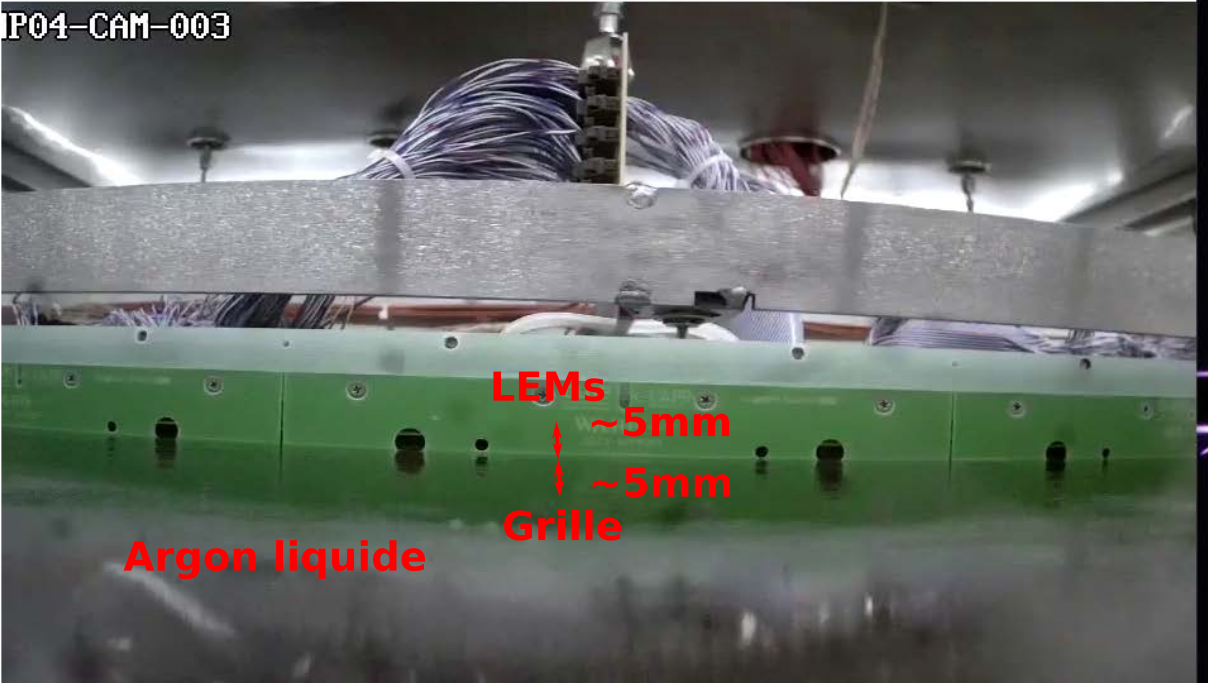
\includegraphics[width=\textwidth]{./pictures/in_coldbox.png}\\
   				CERN, bâtiment 182
    		\end{column}
    		\begin{column}{0.6\textwidth}
    			\begin{scriptsize}
	    			\textbf{Test des CRPs en condition double phase avant leur insertion dans le cryostat du \SSS{}.}\\
	    			
	    			\begin{itemize}
	    				\item[$\bullet$] \textbf{Tension maximum}
	    				\begin{itemize}
	    					\item Grille stable à la \textcolor{red}{valeur nominale de \SI{7.5}{\kilo\volt}}.
	    					\item LEMs stables à \textcolor{red}{3.0--\SI{3.1}{\kilo\volt}}\\
				    					$\Rightarrow$ Gain effectif estimé \textcolor{red}{$\geq 20$}.
	    				\end{itemize}
	    				\item[$\bullet$] \textbf{Stabilité (décharges par heure)}
	    				\begin{itemize}
	    					\item Stable sur plusieurs jours (semaines).
	    					\item \textcolor{red}{1 décharge par heure} par CRP (1 décharge en 36 heures par LEM): \textcolor{red}{ok pour DUN$\nu$E}.
	    					\item \textcolor{red}{1 décharge par heure} $\Rightarrow$ temps mort $\sim$0.3\%.
	    				\end{itemize}
	    				\item[$\bullet$] \textbf{Planéité}
	    				\begin{itemize}
	    					\item \textcolor{red}{\SI{1.2}{\milli\meter}} à travers le CRP : ok.
	    				\end{itemize}
	    			\end{itemize}
	    		\end{scriptsize}
    		\end{column}
    	\end{columns}
	    \end{frame}

    \begin{frame}{Boîte cryogénique au CERN}
        Rajouter une slide avec tension vs time, expliquer que les résultats sont bons
    \end{frame}

       {
       	\setlength\pdfpagewidth{12.8cm}%
       	\setlength\pdfpageheight{11.5cm}%
       	\usebackgroundtemplate{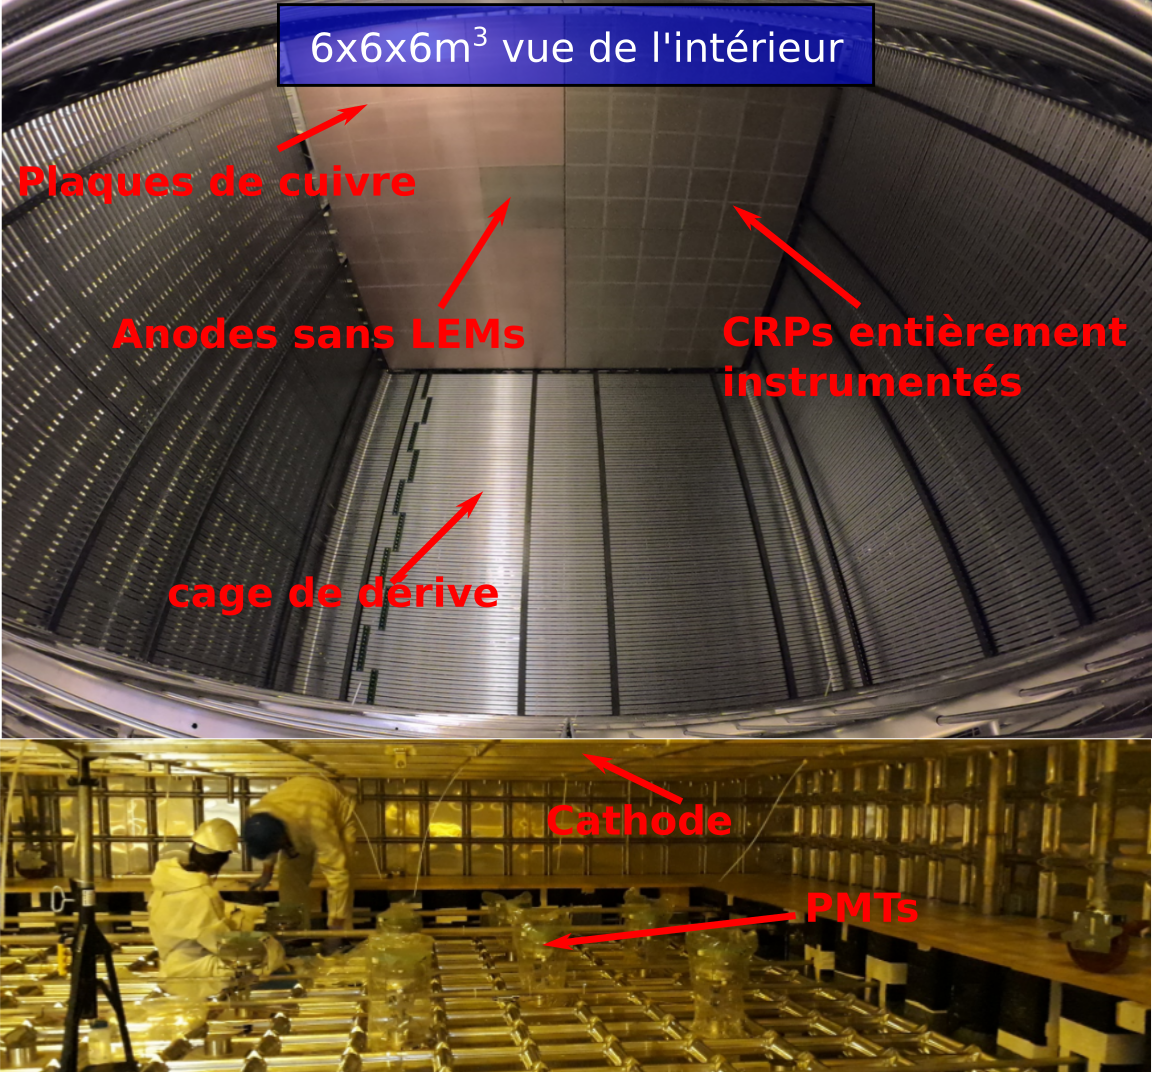
\includegraphics[width=\paperwidth]{./pictures/fisheye.png}}
       \begin{frame}[plain]
       	
       \end{frame}
	    }

    \begin{frame}{État actuel et planning}
        plus de photos (remplissage) et planning
    \end{frame}

    {
    	\usebackgroundtemplate{
\includegraphics[width=\paperwidth]{./pictures/1.pdf}}
        \begin{specialframe}
            \vspace{2cm}\hspace*{-1.8cm}\parbox[t]{\textwidth}{
                \begin{center}
                    \begin{Huge}
                            \textcolor{pheniics_purple}{\textbf{Simulations du CRP et analyse des résultats du \TOO{}}}
                    \end{Huge}
                \end{center}
            }
        \end{specialframe}
    }

    \section[\TOO{}]{Simulations du CRP et analyse des résultats du \TOO{}}

    \begin{frame}{Le prototype de \TOO{}}
		\begin{columns}
			\begin{column}{0.48\textwidth}
				\centering
				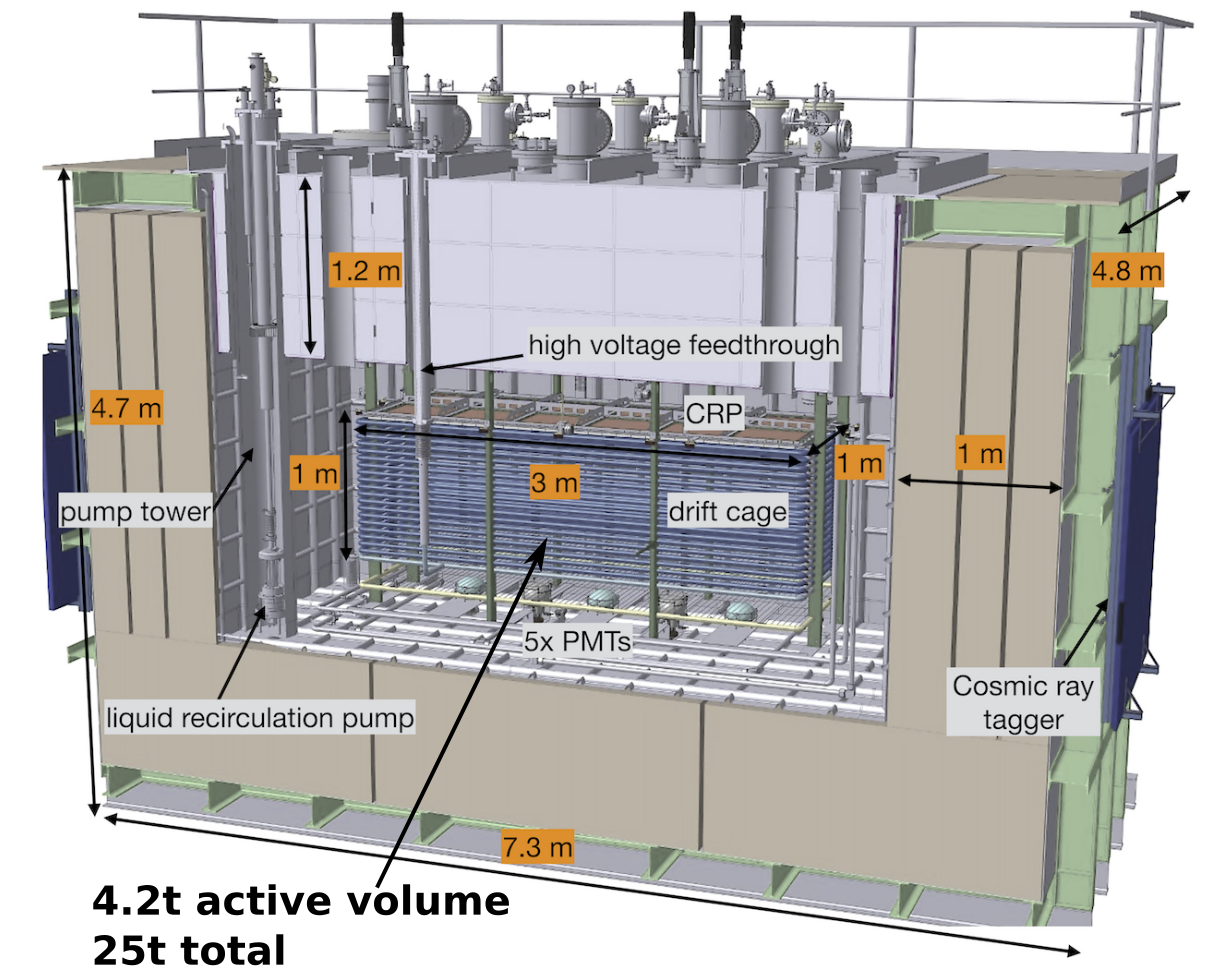
\includegraphics[width=0.8\textwidth]{311_2.png}
			\end{column}\hfill
			\begin{column}{0.48\textwidth}
				\begin{scriptsize}
					\textcolor{red}{Jalon de la technologie DLArTPC :} \\ a montré son fonctionnement à \SI{4}{\tonne}.\\
					Signal/Bruit $\sim$ 10 pour une MIP à une amplification de \SI{28}{\kilo\volt\per\centi\meter}.
				\end{scriptsize}
			\end{column}\hfill
		\end{columns}
		\centering
		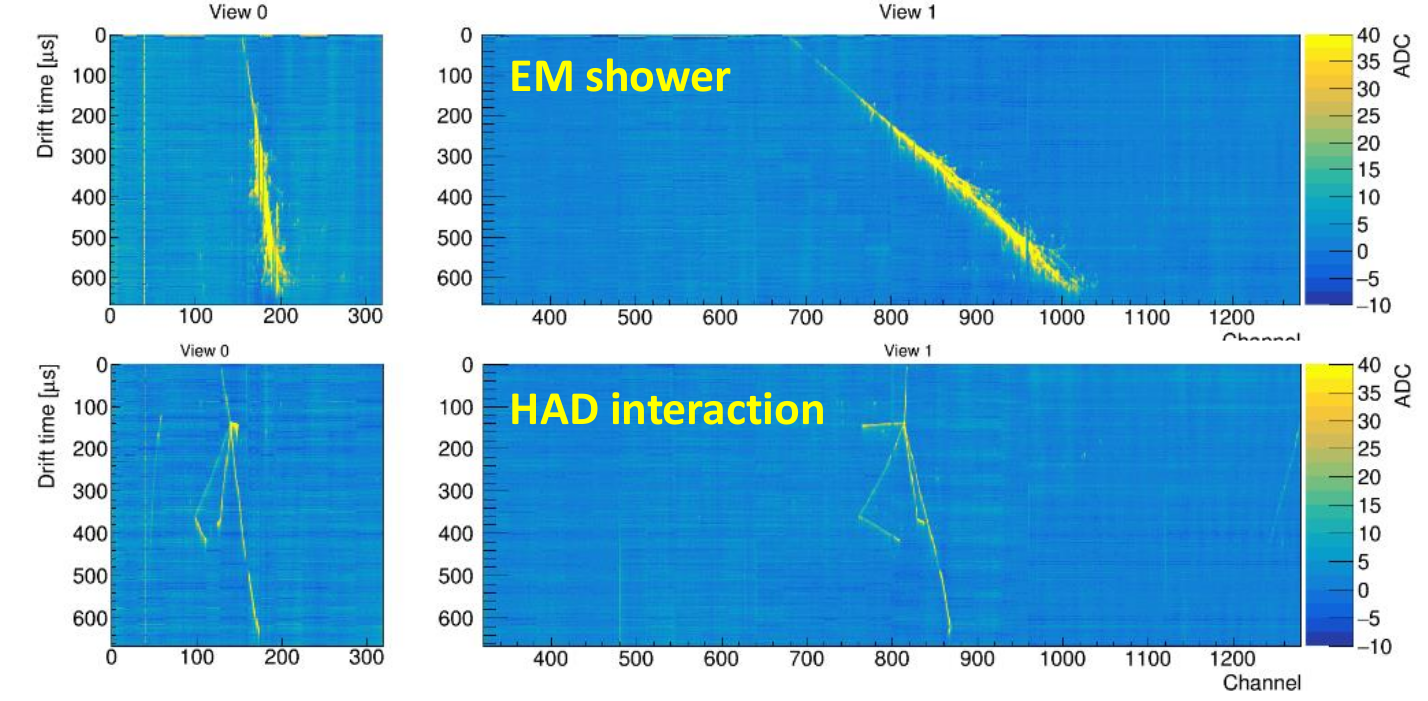
\includegraphics[width=0.77\textwidth]{./pictures/events.png}\\
	\end{frame}
	    
    \begin{frame}{Le prototype de \TOO{}}
    	\begin{scriptsize}
    		\vfill
    		\begin{columns}
    			\begin{column}{0.35\textwidth}
    				Construit en 2016--2017, opéré entre Juin et Novembre 2017.\\
    				\vspace{0.3cm}
    				\textbf{But:} Tester les choix technologiques faits pour le \SSS{}.\\
    				\vspace{0.3cm}
    				\textbf{Difficultés:} 
    				\begin{itemize}
    					\item[$\bullet$] Tension maximum limitée à \SI{5}{\kilo\volt} (nominale : \SI{7}{\kilo\volt})
    					\item[$\bullet$] Haute tension à travers les LEMs instable
    				\end{itemize}
    				\textbf{$\Rightarrow$ Problèmes résolus dans le \SSS{}} \\
    				\vspace{0.3cm}
    				\textbf{Analyse principale :} Gain (vs amplification, vs extraction, stabilité)\\
    				$\Rightarrow$ On regarde les muons cosmiques (MIP).
    			\end{column}\hfill
    			\begin{column}{0.65\textwidth}
    				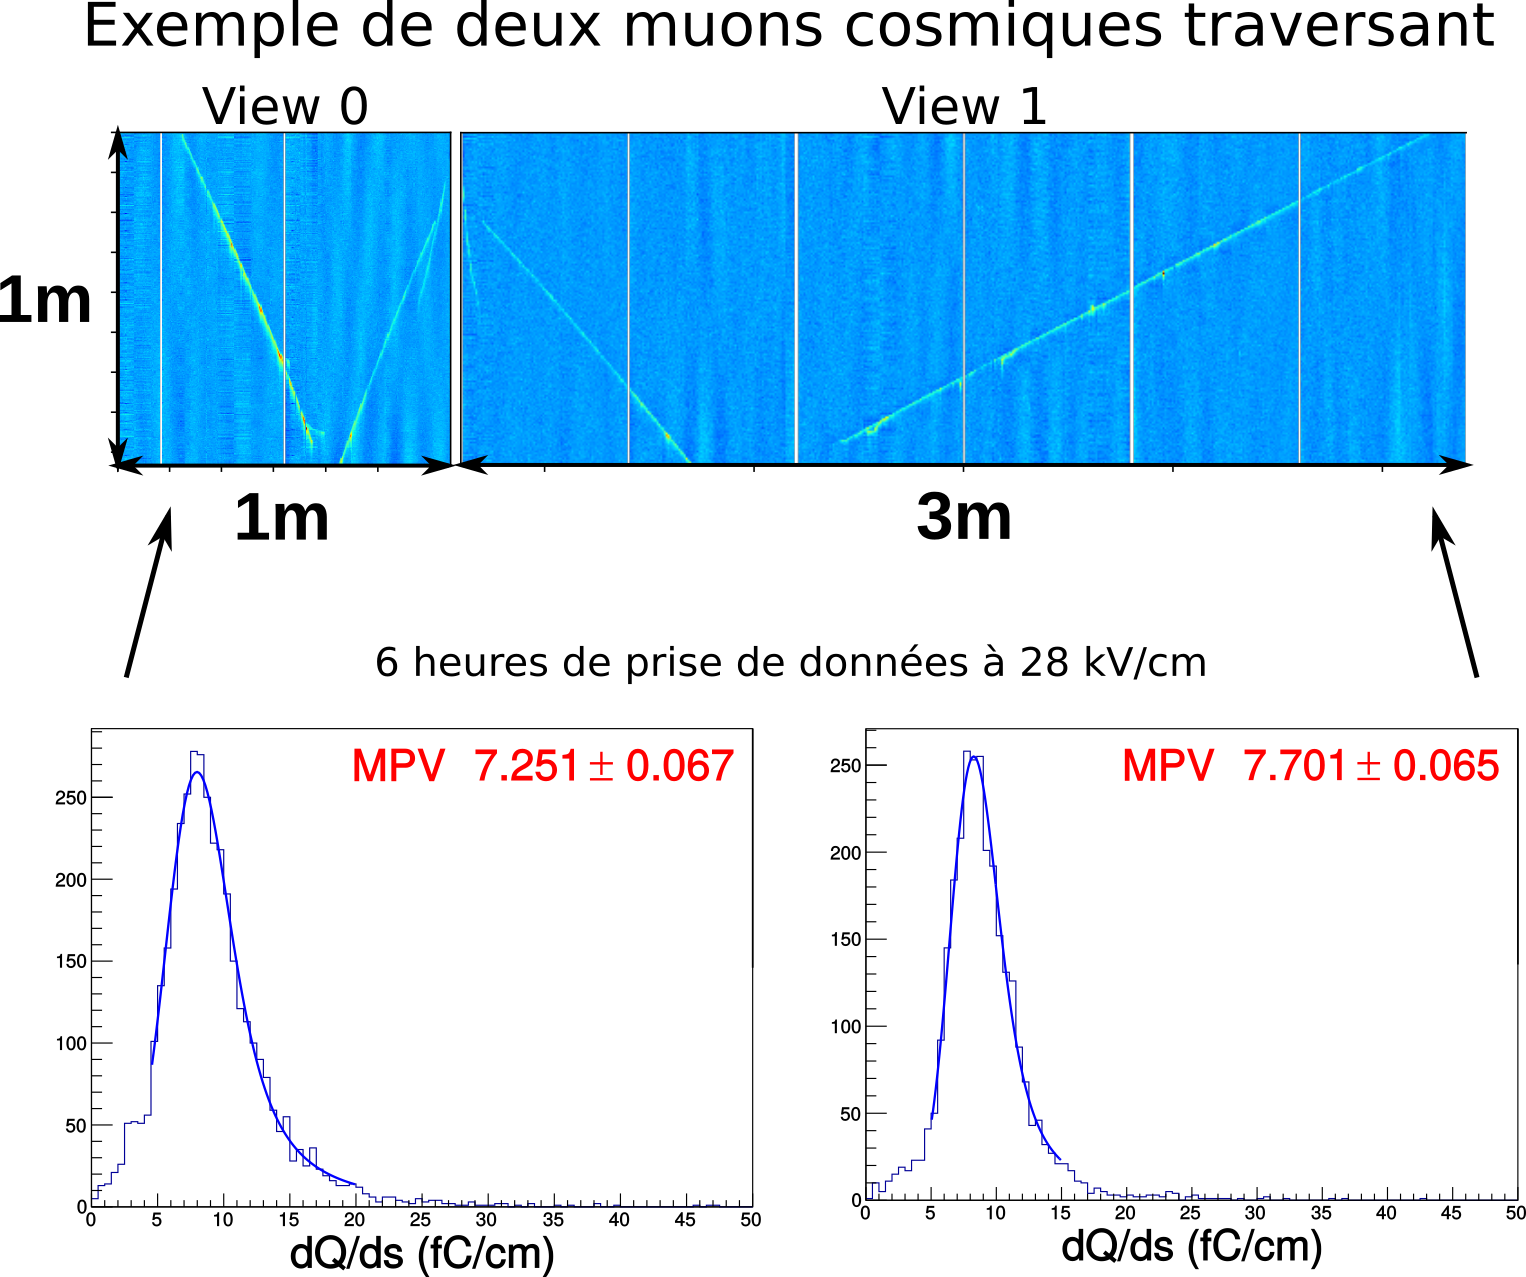
\includegraphics[width=\textwidth]{./pictures/run840.png}\\
    			\end{column}
    		\end{columns}
	    \end{scriptsize}
    \end{frame}

    \subsection{Méthode d'analyse}

    \begin{frame}{Mesure du gain avec des muons cosmiques}
    	\begin{scriptsize}
            \begin{columns}
                \begin{column}{0.6\textwidth}
                    \centering 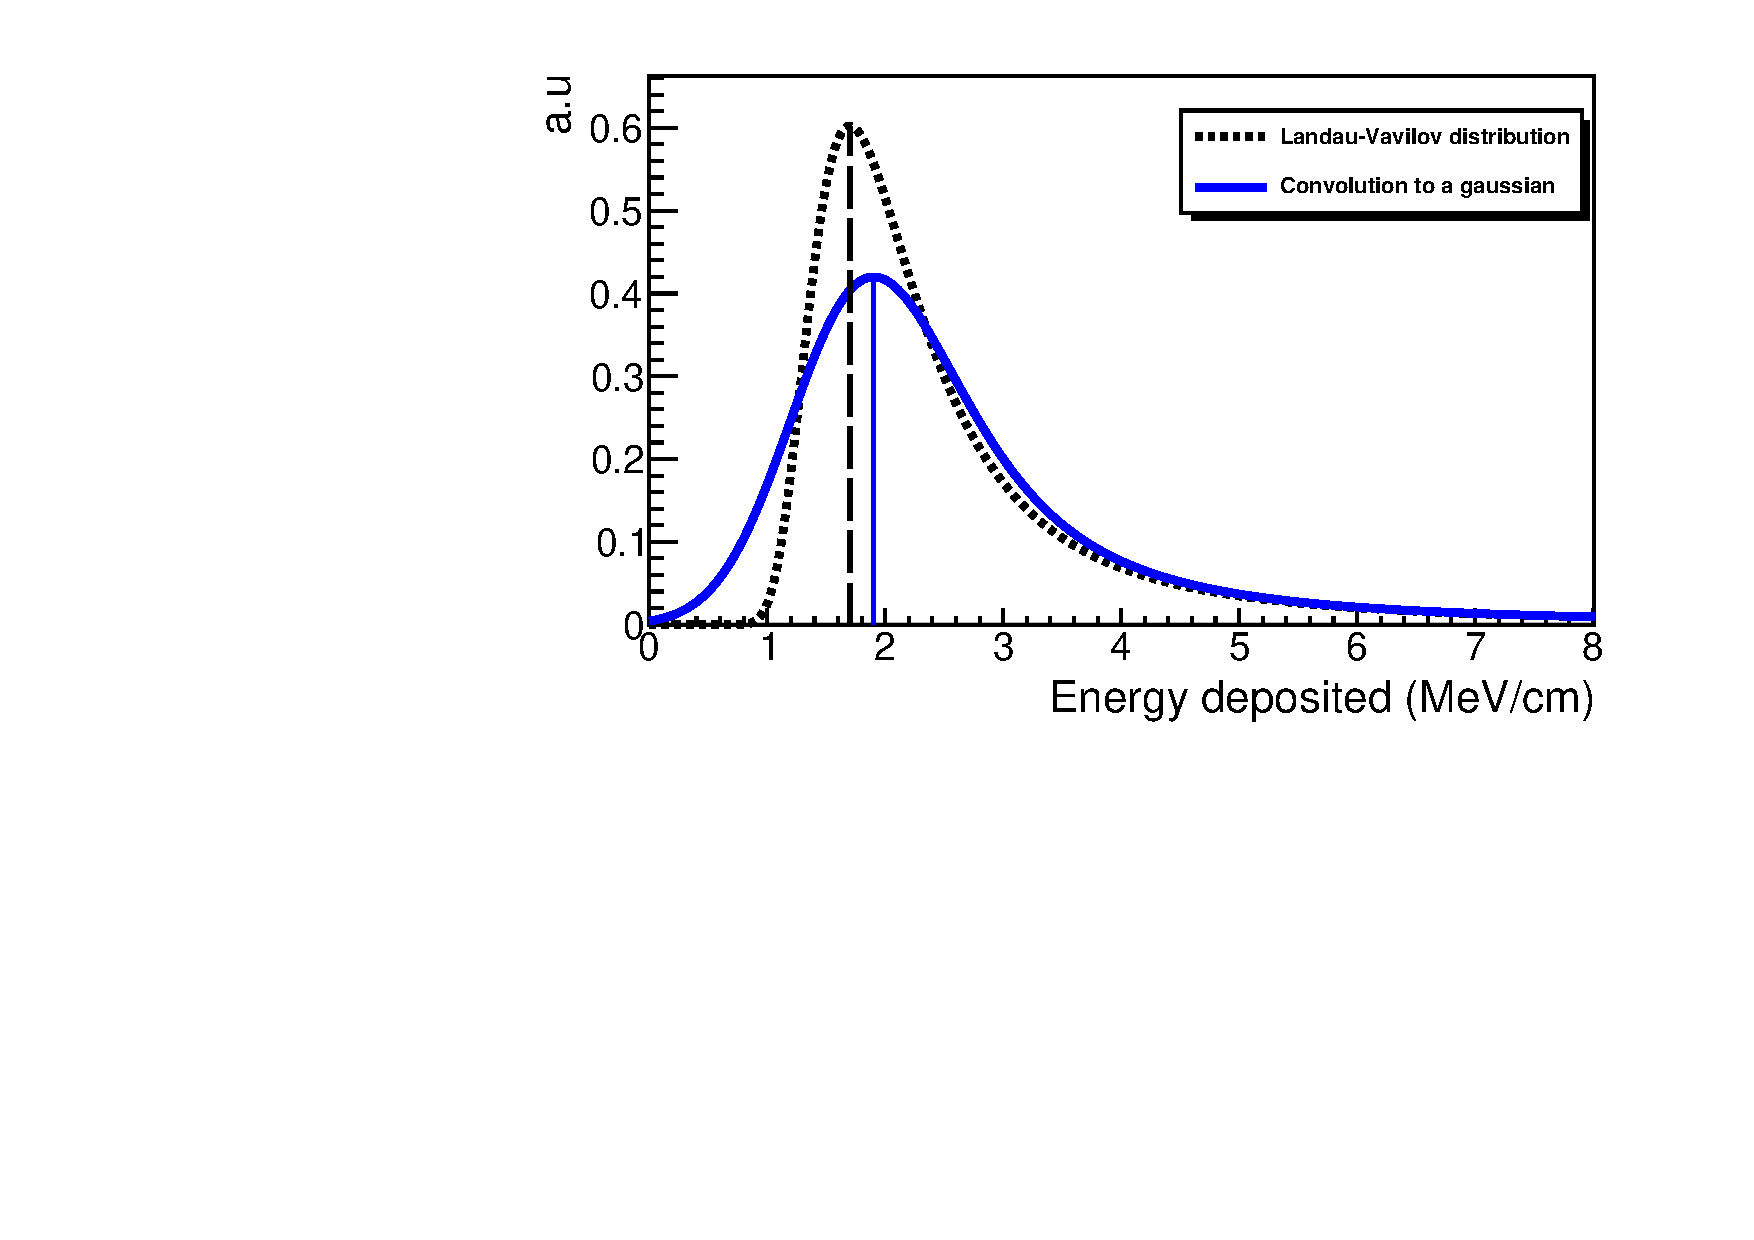
\includegraphics[width=\textwidth]{langau.pdf}
                \end{column}\hfill
                \begin{column}{0.4\textwidth}
                    \begin{itemize}
       					\item[$\bullet$] Muon cosmique : MIP \\ $\Rightarrow$ dépôt d'énergie attendu connu
       					\item[$\bullet$] Valeur la plus probable (MPV) = \SI{1.7}{\mega\electronvolt\per\centi\meter}
       					\item[$\bullet$] Après recombinaison avec les ions (loi de Birk) : \SI{8.26}{\femto\coulomb\per\centi\meter}
       					\item[$\bullet$] $G_{eff}=\frac{MPV_0 + MPV_1}{MPV_{attendue}}$
       				\end{itemize}
                \end{column}
            \end{columns}
            \vspace{0.2cm}
            Calibration de l'électronique du \TOO{} $\Rightarrow$ conversion ADC$\times$temps$\to$\si{\femto\coulomb}
            \begin{center} 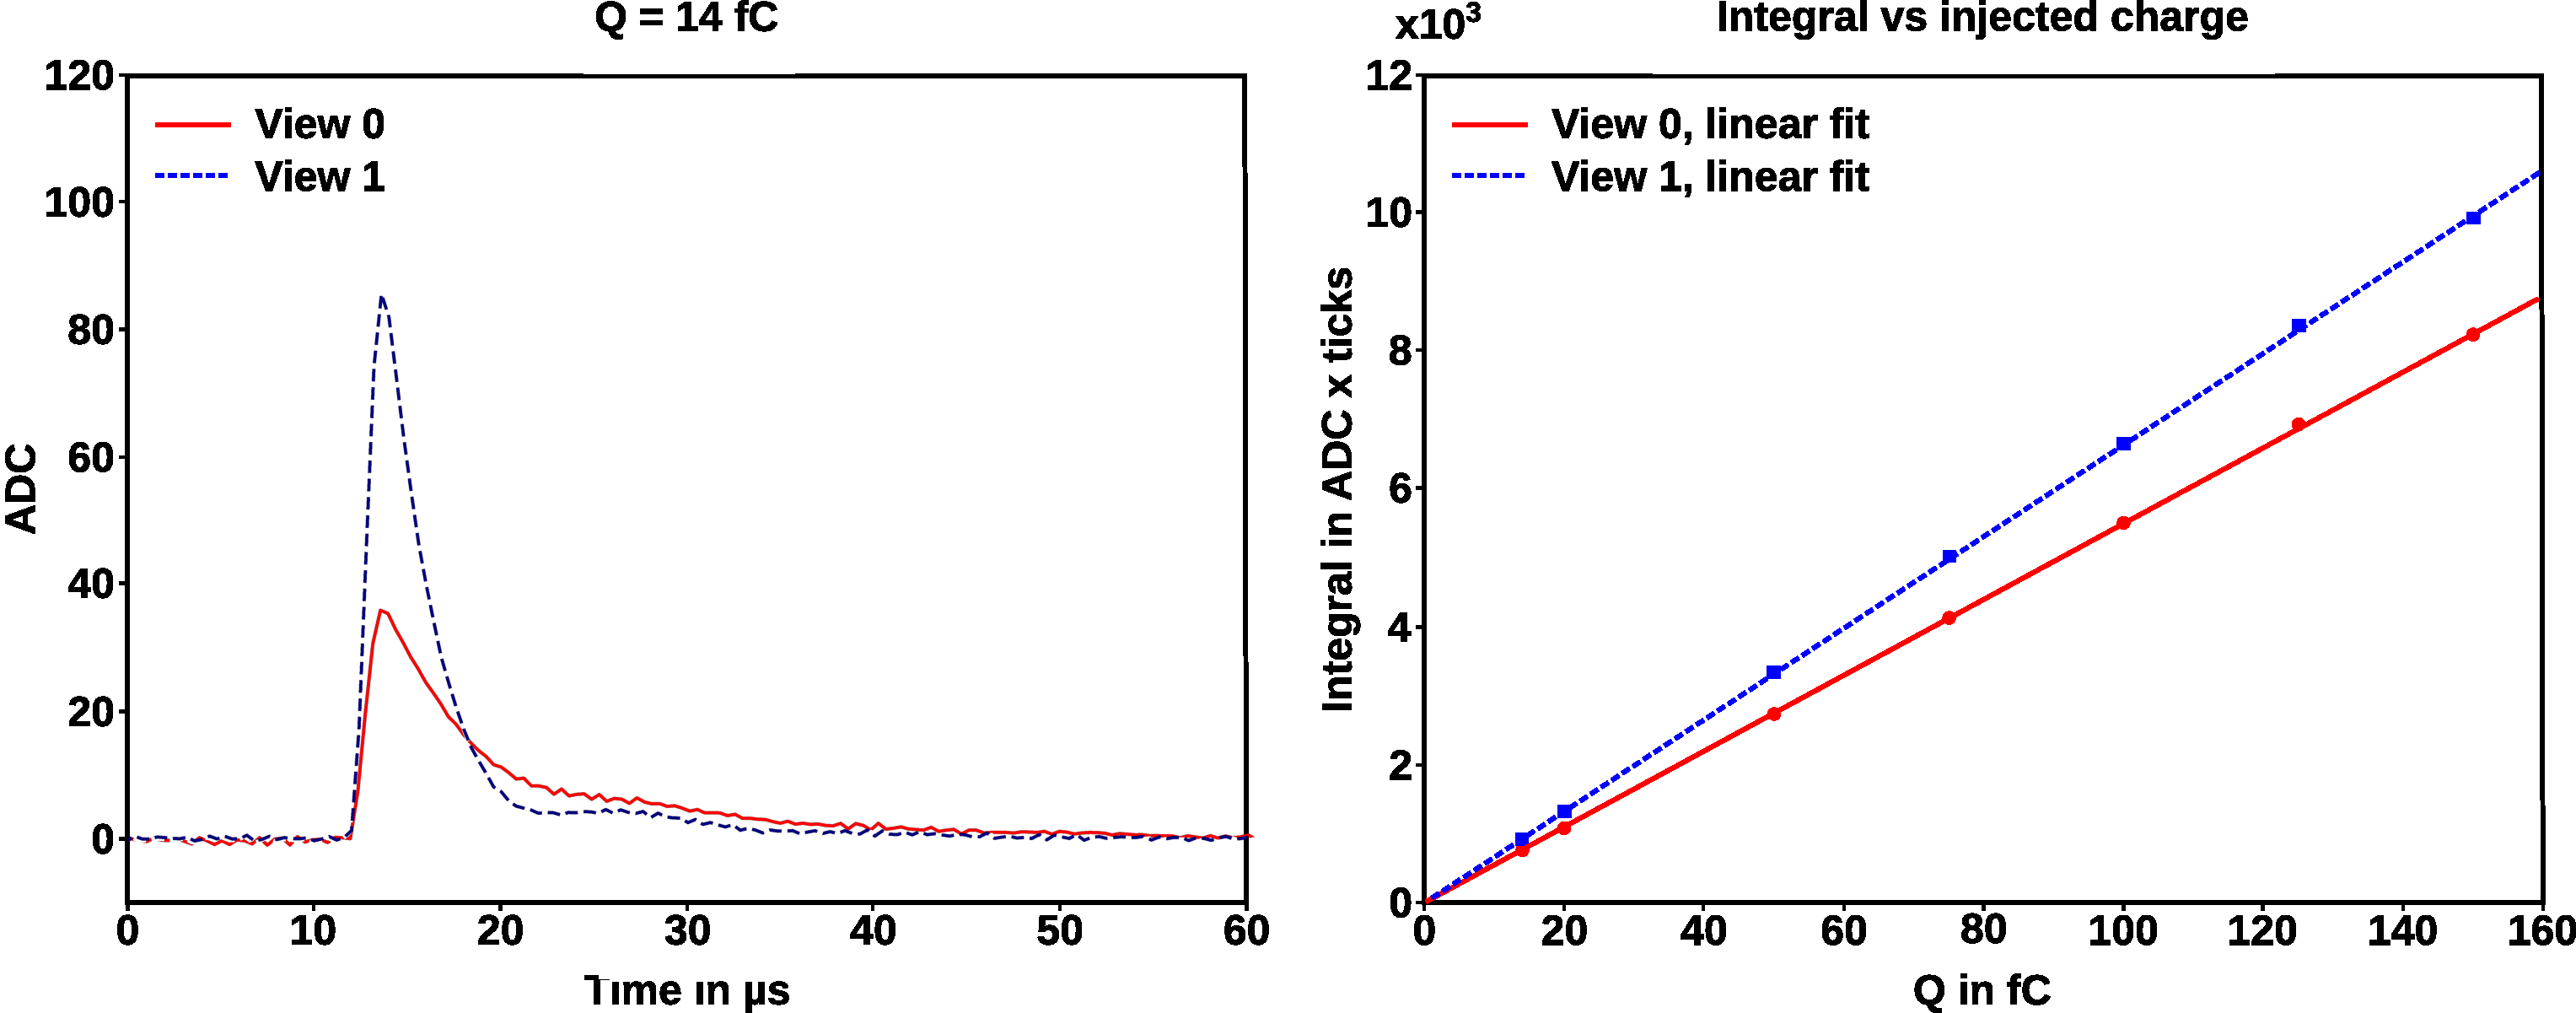
\includegraphics[width=0.8\textwidth]{calibration.pdf} \end{center}
	    \end{scriptsize}
    \end{frame}

    \begin{frame}{Sélection des muons}
        \begin{scriptsize}
        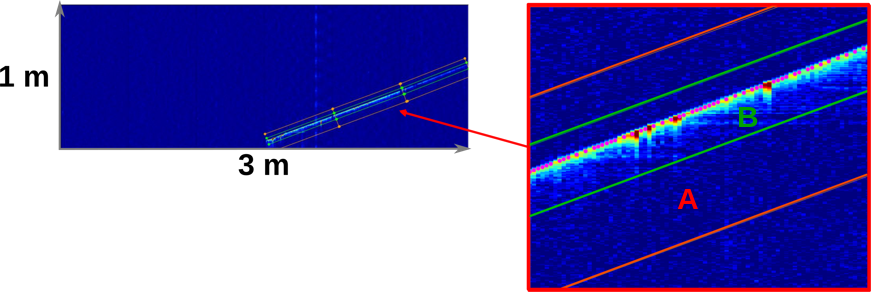
\includegraphics[width=\textwidth]{highway.png}
        \begin{columns}
            \begin{column}{0.5\textwidth}
                \begin{itemize}
                    \item[$\bullet$] Muon : trace longue, droite et nette \\ $\Rightarrow$ Coupure sur $\frac{Q_A-Q_B}{Q_A} < 0.1$
                    \item[$\bullet$] Coupures supplémentaires : \begin{itemize}\begin{scriptsize}\item longueur $>\SI{50}{\centi\meter}$. \item \SI{2}{\degree} autour de la verticale, de l'horizontale, et des directions parallèle aux canaux des anodes.\end{scriptsize}\end{itemize}
                \end{itemize}
            \end{column}
            \begin{column}{0.5\textwidth}
                \begin{itemize}
                    \item[$\bullet$] Efficacité de sélection des muons : 68\,\%
                    \item[$\bullet$] Échantillon final : 92\,\% de muons
                \end{itemize}
            \end{column}
        \end{columns}
        \end{scriptsize}
    \end{frame}

    \subsection[Efficacités de collection]{Efficacités de collection}

    \begin{frame}{Simulation : efficacités de collection}
    	\begin{scriptsize}
    		\begin{columns}
    			\hspace{-1.5cm}
	    		\begin{column}{0.3\textwidth}
	    			\vspace{-2.5cm}
	    			\hbox{
	    				$\mathbf{G_{eff}=G_{LEM}\boldsymbol{\times}\boldsymbol{\epsilon}_{ext} \boldsymbol{\times}\textcolor{red}{\epsilon_{LEM}}\boldsymbol{\times} \textcolor{blue}{\epsilon_{anode}}}$
	    			}\\
	    			\vspace{1.3cm}
	    			\textbf{Difficulté rencontrée dans le $\mathbf{3 \times 1 \times \SI[detect-weight]{1}{\meter\cubed}}$:} Tension de la grille d'extraction limitée à \SI{5}{\kilo\volt}\\
	    			\vspace{0.3cm}
	    			$\Rightarrow$ N'a pas pu opérer à champ d'extraction et d'induction fixés.\\
	    			$\Rightarrow$ Besoin de connaître l'\textcolor{red}{impact} de ces champs \textcolor{red}{sur la collection de charge}.\\
	    			\vfill
%	    			\vspace{0.3cm}	    			
%		    		$\mathbf{G_{eff} = G_{LEM}} $ \\\hspace{0.7cm} $\boldsymbol{\times \epsilon}_{\mathbf{extraction}}$ \\\hspace{0.7cm} \textcolor{red}{$\boldsymbol{\times} \mathbf{P_{LEM}}$}\\\hspace{0.7cm} \textcolor{blue}{$\boldsymbol{\times} \mathbf{P_{Anode}}$}
	    		\end{column}\hfill\hspace{-3.2cm}
	    		\begin{column}{0.65\textwidth}
%	    			\flushright
	    			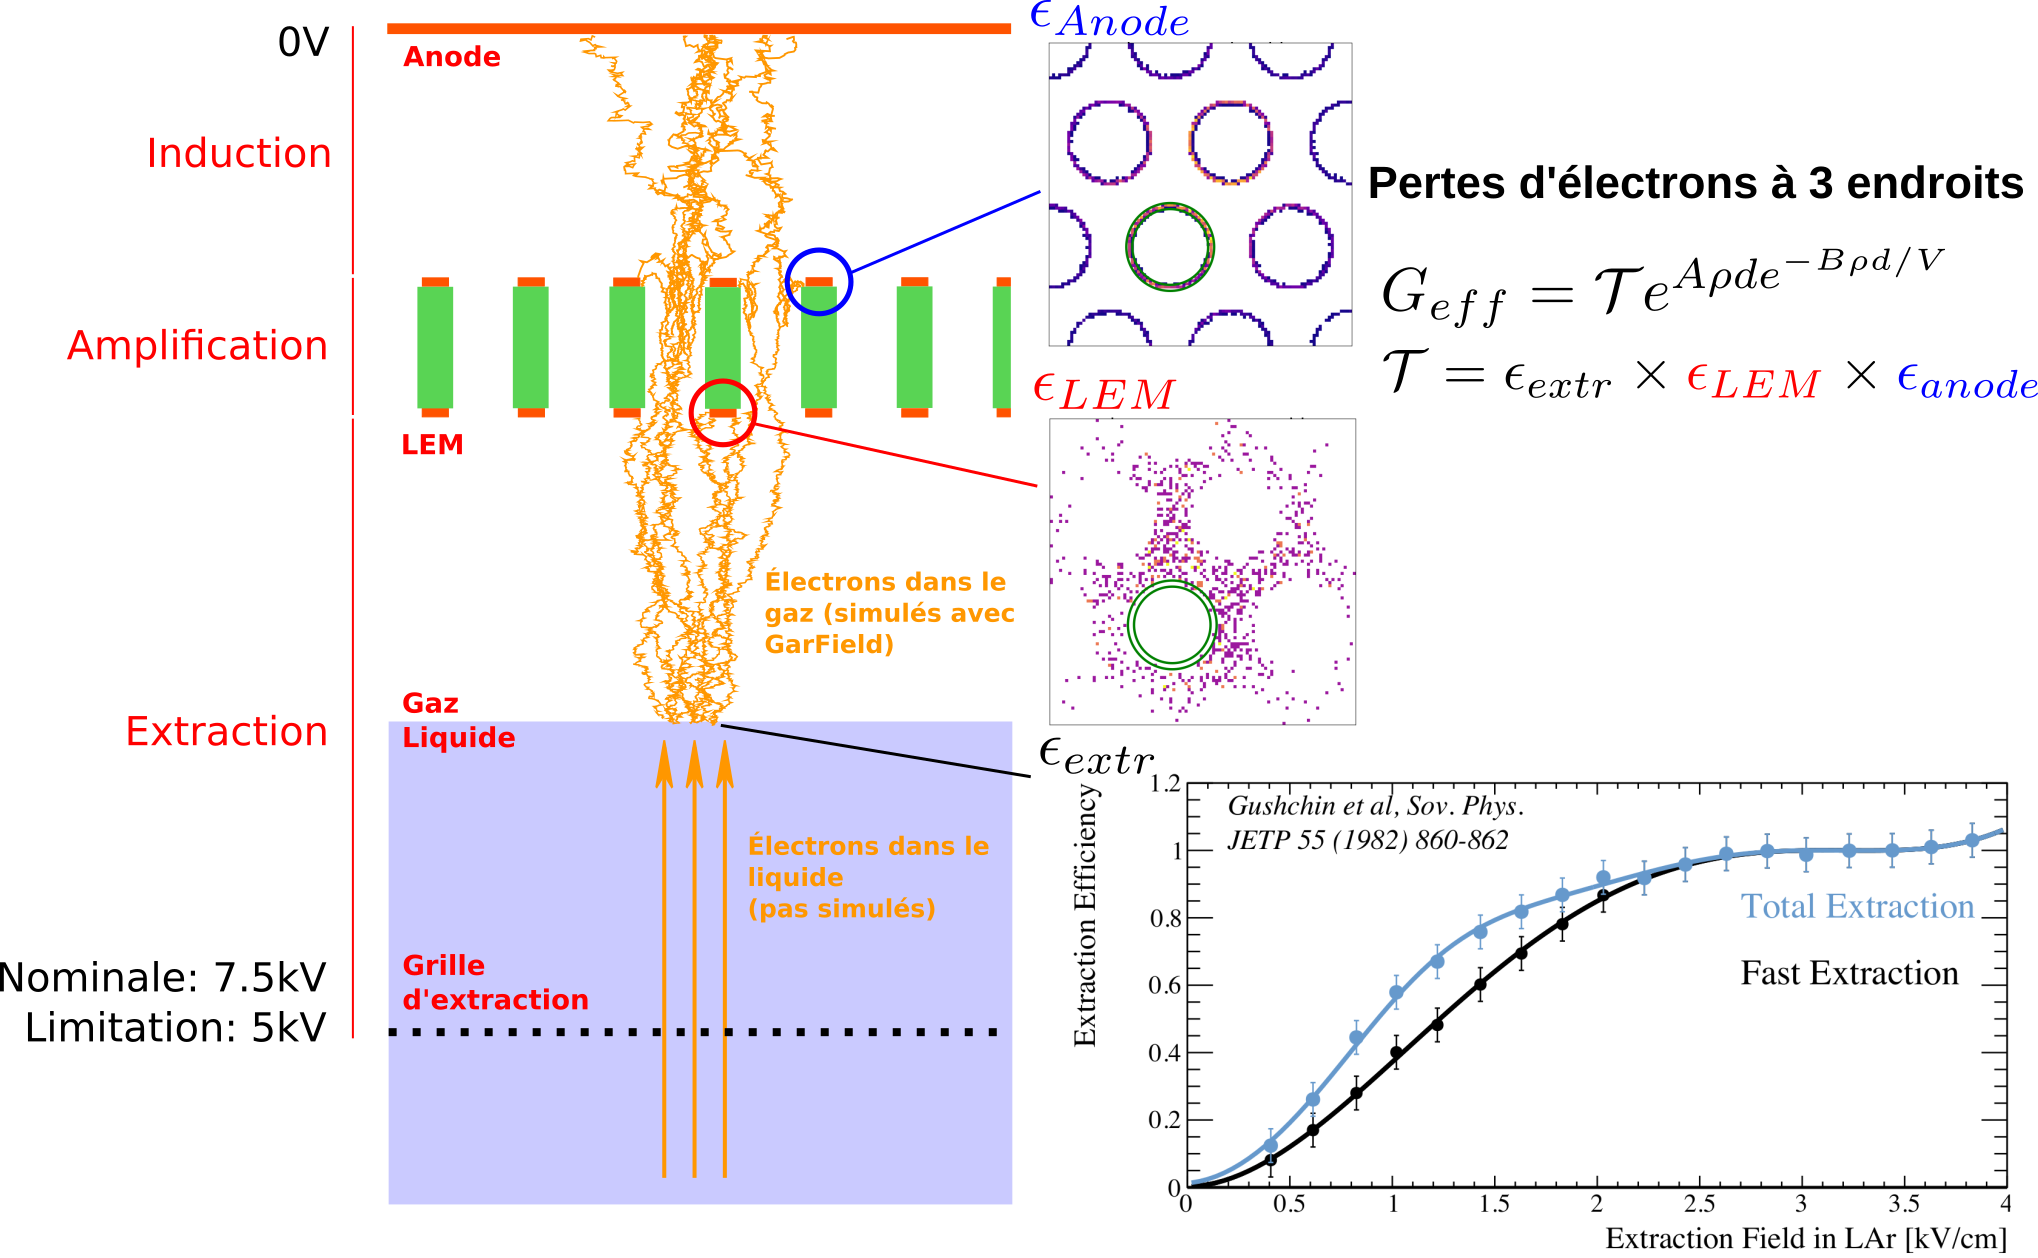
\includegraphics[width=1.18\textwidth]{./pictures/coll_proba_2.png}\\
	    		\end{column}
	    	\end{columns}
    	\end{scriptsize} 
    \end{frame}

    \begin{frame}{Simulation : efficacités de collection}
        \hbox{
     		$\mathbf{G_{eff}=G_{LEM}\boldsymbol{\times}\boldsymbol{\epsilon}_{ext} \boldsymbol{\times}\textcolor{red}{\epsilon_{LEM}}\boldsymbol{\times} \textcolor{blue}{\epsilon_{anode}}}$
     	}
   		\begin{columns}
            \begin{column}{0.5\textwidth}
                \centering $\textcolor{red}{\epsilon_{LEM}}$
                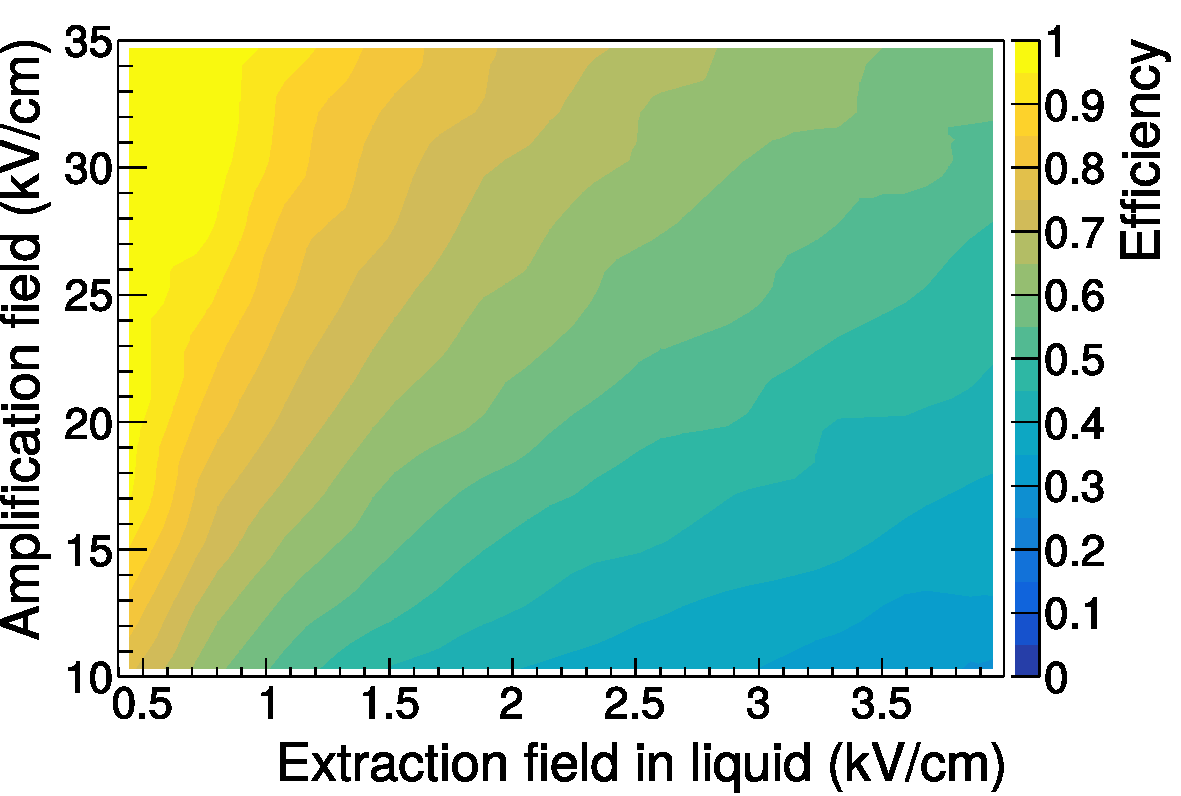
\includegraphics[width=\textwidth]{eff_lem_alone.pdf}
            \end{column}\hfill
            \begin{column}{0.5\textwidth}
                \centering $\textcolor{blue}{\epsilon_{Anode}}$
                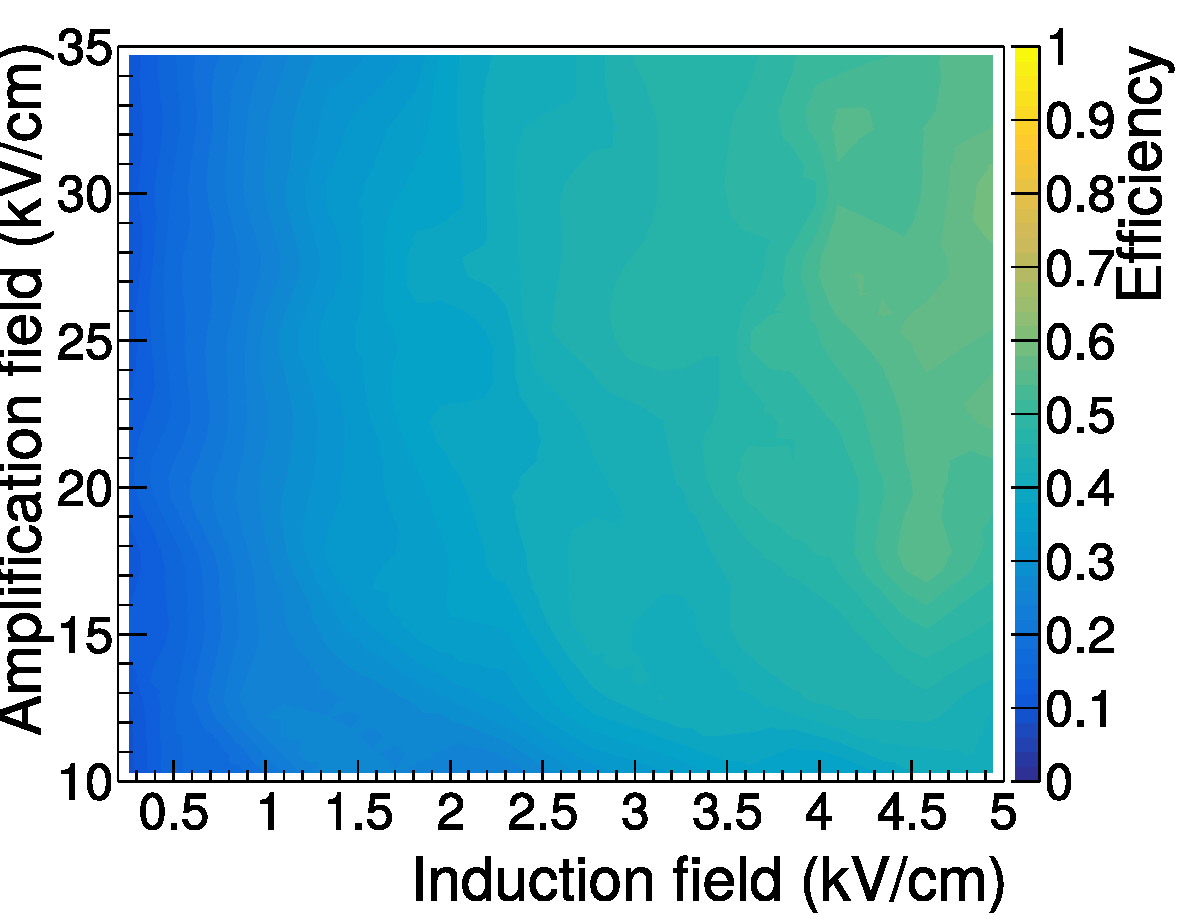
\includegraphics[width=\textwidth]{eff_anode.pdf}
            \end{column}
        \end{columns}
   		\begin{columns}
            \begin{column}{0.5\textwidth}
                \begin{scriptsize}
                    \begin{itemize}
                        \item[$\bullet$] Dépend du champ dans le gaz entre l'interface et le LEM
                        \item[$\bullet$] Champ calculable à partir de la tension grille--LEM et de la position de l'interface
                    \end{itemize}
                \end{scriptsize}
            \end{column}\hfill
            \begin{column}{0.5\textwidth}
                \begin{itemize}
                    \item[$\bullet$] Dépend du charging up du LEM (discuté plus loin)
                    \item[$\bullet$] Simulée ici avant charging up.
                \end{itemize}
            \end{column}
        \end{columns}
    \end{frame}
    
    \begin{frame}{Efficacités de collection : comparaison aux mesures}
        Dans l'enceinte haute pression
        \begin{scriptsize}
            impossible de mesurer les efficacités directement \\$\Rightarrow$ comportement du gain normalisé aux efficacités simulées.
        \begin{columns}
            \begin{column}{0.5\textwidth}
                \centering $\textcolor{red}{\epsilon_{LEM}}$
                \includegraphics[width=\textwidth]{eff_lem_gamelle.pdf}
            \end{column}\hfill
            \begin{column}{0.5\textwidth}
                \centering $\textcolor{blue}{\epsilon_{Anode}}$
                \includegraphics[width=\textwidth]{eff_anode_gamelle.pdf}
            \end{column}
        \end{columns}
   		\begin{columns}
            \begin{column}{0.5\textwidth}
                \begin{itemize}
                    \item[$\bullet$] Pas d'efficacité d'extraction (pas de liquide)
                    \item[$\bullet$] Champ maximum limité par la distance Cathode-LEM et l'alimentation HT
                    \item[$\bullet$] Comportement similaire entre \SI{1}{\kilo\volt\per\centi\meter} et \SI{1.5}{\kilo\volt\per\centi\meter}
                \end{itemize}
            \end{column}\hfill
            \begin{column}{0.5\textwidth}
                \begin{itemize}
                    \item[$\bullet$] Comportement similaire, mais différences allant jusqu'à 15\,\%
                \end{itemize}
            \end{column}
        \end{columns}
        \end{scriptsize}
    \end{frame}

    \begin{frame}{Efficacités de collection : comparaison aux mesures}
        Dans le \TOO{}
        \begin{scriptsize}
            \begin{columns}
                \begin{column}{0.5\textwidth}
                    \includegraphics[width=\textwidth]{./pictures/gain_vs_extr.pdf}
                \end{column}
                \begin{column}{0.5\textwidth}
                    \includegraphics[width=\textwidth]{./pictures/comp_311_eff.pdf}
                \end{column}
            \end{columns}\vspace{0.5cm}
            \begin{columns}
                \begin{column}{0.5\textwidth}
                    \begin{itemize}
                        \item[$\bullet$] Champs d'amplification (\SI{28}{\kilo\volt\per\centi\meter}) et d'induction (\SI{1}{\kilo\volt\per\centi\meter}) constants
                        \item[$\bullet$] Grandes barres d'erreur à faibles champs dues aux imperfections de la planéité
                    \end{itemize}
                \end{column}
                \begin{column}{0.5\textwidth}
                    \begin{itemize}
                        \item[$\bullet$] MPV Normalisée à $\epsilon_{extr}$ à \SI{2}{\kilo\volt\per\centi\meter} pour comparer le comportement
                        \item[$\bullet$] La MPV divisée par  $\epsilon_{LEM}$ est plus en accord avec $\epsilon_{extr}$ que la MPV seule.
                    \end{itemize}
                \end{column}
            \end{columns}
        \end{scriptsize}
    \end{frame}

    \begin{frame}{Efficacités de collection : impact sur la précision du gain}
        \begin{center} \vspace{-0.5cm}\includegraphics[width=\textwidth]{CRP-metrologie.png} \end{center}
        \begin{scriptsize}
            \begin{columns}
                \begin{column}{0.6\textwidth}
                    \centering \includegraphics[width=\textwidth]{./pictures/extr_eff.pdf}
                \end{column}\hfill
                \begin{column}{0.4\textwidth}
                    \begin{itemize}
       					\item[$\bullet$] Déformation du CRP : $\pm\SI{1.8}{\milli\meter}$
       					\item[$\Rightarrow$]  25\,\% variation des champs entre la grille et l'interface et entre l'interface et les LEMs
       					\item[$\bullet$] Variation de $\epsilon_{extr}\times\epsilon_{LEM}$ à basse tension d'extraction
       				\end{itemize}
                     \textbf{Note : } dans le \SSS{}, la tension Grille-LEM $\sim\SI{2.5}{\kilo\volt}$ fait que l'efficacité sera $\sim$ constantes avec le champ électrique.
                \end{column}
            \end{columns}
        \end{scriptsize}
    \end{frame}

    \begin{frame}{Stabilité du gain à travers le CRP dans le \TOO{}}
        \begin{scriptsize}
            \centering Deux runs à 12 heures d'intervalle. Extraction \SI{1.9}{\kilo\volt\per\centi\meter}, Amplification \SI{28}{\kilo\volt\per\centi\meter}, Induction \SI{1.5}{\kilo\volt\per\centi\meter}\\\vspace{0.2cm}
            \begin{center} \vspace{-0.5cm}\includegraphics[width=0.9\textwidth]{dQds_2D_840.pdf} \end{center}
            \begin{center} \vspace{-0.5cm}\includegraphics[width=0.9\textwidth]{dQds_2D_842.pdf} \end{center}
            \vspace{-0.5cm}
            \begin{itemize}
    			\item[$\bullet$] Variations attendues dues aux variations d'épaisseur et à la planéité du CRP : $\pm 12 \,\%$
    			\item[$\bullet$] Variations observées jusqu'à $\sim \pm15\,\%$ : compatibles
			\end{itemize}
        \end{scriptsize}
    \end{frame}

  \subsection{Charging up}

    \begin{frame}{Charging up}
    	\begin{scriptsize}
    		\begin{columns}
    			\begin{column}{0.5\textwidth}
    				\includegraphics[width=0.85\textwidth]{CU.png}\\
                    \vspace{0.1cm}
    				\includegraphics[width=\textwidth]{3L_charging_up.png}\\
    				\includegraphics[width=0.7\textwidth]{gain_3L.pdf}
    			\end{column}\hfill
    			\begin{column}{0.5\textwidth}
    				\begin{itemize}
    					\item[$\bullet$] Lignes de champ traversent le FR4\\
    					$\Rightarrow$ L'accumulation d'électron \textcolor{blue}{déforme et atténue} le champ
    					\item[$\bullet$] Charging up: \textcolor{red}{$G_{eff}(t)$ décroît} jusqu'à un plateau.
%    					\item[$\bullet$] Le temps de charging up time dépend de la tension dans le LEM et du taux de dépôt de charge.
    				\end{itemize}
    				\vspace{0.3cm}
    				\begin{itemize}
    					\item[$\bullet$] Simulation de $\textcolor{blue}{\epsilon_{Anode}}$ suppose un LEM \textcolor{red}{avant charging up}
    					\item[$\bullet$] Mesures de gain dans l'enceinte faites \textcolor{red}{après charging up}
    					\item[$\bullet$] Mesures de gain dans le \TOO{} faites \textcolor{red}{pendant le charging up}
    					\item[$\Rightarrow$] $\textcolor{blue}{\epsilon_{Anode}}$ simulée sera plus faible que dans le \TOO{} (moins de pertes dues au charging up). Mais ce qui compte vraiment est le \textbf{comportement} de $\textcolor{blue}{\epsilon_{Anode}}$
    				\end{itemize}
    			\end{column}
    		\end{columns}
    	\end{scriptsize}
    \end{frame}

   \begin{frame}{Charging up dans le \TOO{}}
        \begin{scriptsize}
            \includegraphics[width=\textwidth]{charging_up.png}
            \begin{itemize}
                \item[$\bullet$] Charging up $\sim$ linéaire sur les durées des runs du \TOO{}
                \item[$\bullet$] Persiste une fois la tension coupée
            \end{itemize}
        \end{scriptsize}
    \end{frame}

  \subsection{Zones mortes}
    
    \begin{frame}{Simulations : zones mortes}
    	\begin{scriptsize}
    		\begin{minipage}{0.38\textwidth}
    			\begin{center}
    				\includegraphics[width=0.8\textwidth]{corner_annotations.png}\\
    				design : CFR-34\\
    			\end{center} 
    			Zones mortes = zones sans trous d'amplification:
    			\begin{itemize}
    				\item[$\bullet$] Bords du LEM
    				\item[$\bullet$] Trous des vis.
    				\item[$\bullet$] Connecteurs haute tension.
    			\end{itemize}
    			$\Rightarrow$ Collection de charge?\\
    			$\Rightarrow$ Résolution en énergie?\\
    			
    			\textbf{ANSYS} simule la carte de champ à travers le CRP.\\
    			\textbf{GarField} simule la dérive des électrons dans cette carte.\\
    		\end{minipage}
    		\begin{minipage}{0.58\textwidth}
    			\centering
    			\includegraphics[width=0.8\textwidth]{drift_example.png}\\
    			\vspace{0.5cm} \hspace{0.1cm}
    			\begin{minipage}{0.48\textwidth}
    				\centering
    				\textbf{Carte d'efficacité du LEM}\\
    				\includegraphics[width=\textwidth]{eff_map.png}
    			\end{minipage}\hfill
    			\begin{minipage}{0.48\textwidth}
    				\centering
    				\textbf{Impact sur la charge vue dans le} $\mathbf{6 \times 6 \times 6} \,\textbf{\si[detect-weight]{\meter\cubed}}$\\
    				\includegraphics[width=\textwidth]{electron.png}
    			\end{minipage}
    		\end{minipage}
    	\end{scriptsize} 
    \end{frame}

    \begin{frame}{Zones mortes dans le \TOO{}}
        comparaison 311\\
        Un mot sur le 666
    \end{frame}

  \subsection{Gain vs amplification}

    \begin{frame}{Gain vs amplification}
        % PLUS POSITIF : Ont voit qu'on est pas loin du 3L, charging up semble fini, comportement ok, gain attendus a HT compatibles avec nos besoins
        \begin{scriptsize}
            \begin{columns}
                \begin{column}{0.5\textwidth}
                    \includegraphics[width=\textwidth]{./pictures/gain_vs_ampli.pdf} \\ 
                    \begin{itemize}
                        \item[$\bullet$] \TOO{} \textcolor{red}{légèrement sous les résultats} du \threeL{} après charging up, sauf au delà de \SI{28}{\kilo\volt\per\centi\meter}.
                        \item[$\bullet$] Run à \SI{28}{\kilo\volt\per\centi\meter} fait plus tôt : charging up incomplet.
                    \end{itemize}
                \end{column}
                \begin{column}{0.5\textwidth}
                    \begin{itemize}
                        \item[$\bullet$] État du charging up inconnu dans le \TOO{}
                        \item[$\Rightarrow$]  \textcolor{red}{Devrait être entre les résultats du \threeL{} avant et après charging up}
                    \end{itemize}
                    \begin{itemize}
                        \item[$\bullet$] \textcolor{red}{Run au delà de \SI{28}{\kilo\volt\per\centi\meter}} : très grandes barres  d'erreurs 
                           \begin{itemize}
                                \begin{scriptsize}
                                    \item Plus grand champ d'ampli $\Rightarrow$ plus grand impact des variations d'épaisseurs des LEMs
                                     \item Plus faible champ d'extraction ($\sim \SI{1}{\kilo\volt\per\centi\meter}$) $\Rightarrow$ plus grand impact des imperfections de planéité
                                    \item[$\bullet$] Reconstruits avec une autre méthode que les autres runs (décrite plus loin)
                                \end{scriptsize}
                            \end{itemize}
                    \end{itemize}
                \end{column}
            \end{columns}\vspace{0.2cm}
            $\Rightarrow$ Beaucoup de corrections appliquées pour calculer le gain : beaucoup d'incertitudes systématiques.\\
            $\Rightarrow$ $\epsilon_{Anode}$ avant charging up utilisée, alors que le \TOO{} est en cours ou après charging up.
        \end{scriptsize}
    \end{frame}

    \begin{frame}{Gain vs amplification}
        Meme qu'avant mais entoure les deux points a haute tension\\
        Ces points sont importants car sont aux tensions auxquelles ont veut fonctionner dans le 666\\
        Haute amplification -> basse extr et ind -> difficultés de reco -> dvpt d'un algo dédié\\
    \end{frame}

    \begin{frame}{Reconstruction avec LArSoft}
        LArSoft methode et pbm pour ces runs : \\
        Réduc' bruit en plusieurs passes avant reco des traces\\
        Utilise amas.\\
        Or ces runs ont des low hit -> pas vu -> pleins d'amas -> plusieurs petites traces\\
        dQ/ds
    \end{frame}

    \begin{frame}{Reconstruction avec la transformation de Hough}
        Mon algo : Utilise transformation de Hough -> peu importe les gap entre les hits, on cherche des DROITES \\ A ses propres désavantages (prochain slide) \\
        Une fois traces trouvées, refait la suppression du bruit cohérent en sachant où sont les traces -> récupère des hits et donc de la stat.
    \end{frame}

    \begin{frame}{Reconstruction avec la transformation de Hough}
        Transfo de Hough et illustration
    \end{frame}

    \begin{frame}{Reconstruction avec la transformation de Hough}
        dQds LQrSoft vs Hough
    \end{frame}

  \subsection{Lumière}

    \begin{frame}{Lumière}
        Un slide sur la lumière
    \end{frame}

  \section{Conclusion}

    \begin{specialframe}
        \vspace{2cm}\hspace*{-1.8cm}\parbox[t]{\textwidth}{
            311 ok \\
            perpectives pour le 666 : space charge, Ion feedback, montrer events si il y en a
        }
    \end{specialframe}
    
\end{document}
